\title{Quantitative Easing and Global Oil Futures: The Unseen Market Choreography}
\author{Noah Sidoli \\ Telfer School of Management \\ University of Ottawa \\ \\ Supervisor: Dr. Fabio Moneta}
\date{August 2024}

\documentclass{article}
\usepackage{array}
\newcolumntype{C}{>{\centering\arraybackslash}X}
\usepackage{graphicx}
\usepackage{parskip}
\usepackage{caption}
\usepackage{tablefootnote}
\usepackage{hyperref}
\usepackage{tabularx}
\usepackage{adjustbox}
\usepackage[a4paper, margin=1.5in, top=1.5in]{geometry}
\usepackage{longtable}
\usepackage{ltablex} 
\keepXColumns
\usepackage{amsmath}
\usepackage{float}
\usepackage{booktabs}
\usepackage{amsmath}
\usepackage{multirow}
\usepackage{siunitx}
\usepackage[style=authoryear]{biblatex}
\addbibresource{References.bib}
\DefineBibliographyStrings{english}{%
  bibliography = {References},
}
\setlength{\bibitemsep}{1em} % Adjust the value as needed


\begin{document}

\maketitle

\begin{abstract}
This study examines the impact of unconventional monetary policies, specifically quantitative easing (QE) and quantitative tightening (QT), on daily WTI and Brent futures return. Focusing on announcements from the Great Recession to COVID-19 by the Federal Reserve, European Central Bank, and Bank of England, the research investigates how these policies influence the daily returns of oil futures. Key transmission channels, such as foreign exchange, economic expectations, supply, and investor displacement, are highlighted. Empirical evidence shows that Federal Reserve LSAP announcements primarily affect WTI futures the day after through the exchange rate and economic expectation channels, with effects of -2.95 and -0.16 log percentage points, respectively. Similar effects are observed for Bank of England and European Central Bank announcements on Brent Crude futures. Additionally, open interest changes in oil futures contracts surrounding policy announcements show greater variability for easing announcements compared to tightening suggesting there is more economic uncertainty surrounding oil when QE is announced.
\end{abstract}

\newpage
\tableofcontents
\newpage
        
\section{Introduction}
In recent years, the global economy has witnessed significant shifts in monetary policy strategies, particularly with the introduction of unconventional measures such as quantitative easing (QE) put into practice less than two decades ago in developed economies. This departure from traditional monetary policies has sparked considerable interest and debate among economists and policymakers alike. One area that has garnered attention is the impact of these unconventional methods of monetary policy on commodity prices, with particular emphasis on oil, the lifeblood of the global economy. 

While conventional monetary policy tools have long been studied for their effects on commodity prices, the introduction of QE presents a unique avenue for exploration. QE initiatives, introduced by central banks in the aftermath of the 2007-2008 financial crisis, have been instrumental in driving rapid recoveries in commodity prices, especially in the case of oil. The significance of oil prices as a key indicator of economic activity underscores the importance of understanding the ramifications of QE on these prices (Ratti \& Vespignani, 2013). Quantitative easing done by central banks following the 2007-08 crisis was important in the recovery of oil prices, a trend that imposed a longer recovery time for the economy as a whole (Yoshino et al., 2014). Conventional hypotheses suggest that tightening monetary policy or tapering QE programs should lead to lower oil prices. However, the intricate relationship between periods of quantitative tightening and oil price movements warrants a more nuanced investigation (Yang et al., 2023). 

It is important to recognize that there exists multiple channels in which monetary easing can affect oil prices specifically futures. These channels include the exchange rate, economic expectations, investor displacement, and inventory channels. Understanding these transmission mechanisms is crucial for discerning the impact of monetary policy decisions on commodity markets (Miranda-Pinto et al., 2023). For futures contracts, the cost of carry channel affects the implicit cost of storing the commodity, while the real economy channel influences current and future commodity consumption decisions (Miranda-Pinto et al., 2023). Recent studies have highlighted the role of monetary policy in influencing the immediate production and stockpiling of commodities, particularly during periods of easing (Anzuini et al., 2013). The Federal Reserve's large-scale asset purchase (LSAP) programs, such as LSAP 1 and LSAP 2, have demonstrated substantial impacts on energy prices equivalent to unanticipated cuts in the federal funds target rate of 156 basis points (Rosa, 2014). 

The significance of oil and its price fluctuations in the global economy has long been a focal point for empirical research. These fluctuations hold substantial weight in shaping economic recessions and influencing production growth, particularly within the United States (Barsky \& Killian, 2004). The events of 2020, catalyzed by the COVID-19 pandemic, proved a difficult period for energy prices. With the travel sector representing a staggering 66 percent of all U.S. oil consumption, the industry faced unprecedented challenges during pandemic-induced lockdowns. April 20th, 2020 marked a historic moment for U.S. oil benchmark West Texas Intermediate (WTI) that saw the front month contract price decrease from \$18 to approximately \$-37 per barrel. Similarly, Brent Crude, a global benchmark for oil, saw its futures contract decline to \$9.21 on April 21st, constituting an 86 percent decrease from the beginning of 2020. This price action underscored the severity of the exogenous demand shock that reverberated throughout the energy sector. The onset of these crises was foreshadowed by significant monetary policy action across North America and the Europe. Just over a month before the oil benchmarks went negative, on March 15, 2020, the U.S. Federal Reserve announced its intent to purchase at least \$500 billion in Treasury securities and \$200 billion in government-guaranteed mortgage-backed securities, alongside a cut in the federal fund's target rate window to a quarter percent.

The roots of this research interest can be traced back to Hamilton's pivotal 1983 paper, which explored the correlation between oil prices and macroeconomic fluctuations, particularly during recessionary periods. Hamilton's findings highlighted a recurring pattern wherein oil price shocks often precede U.S. recessions post-World War II. Further research, notably by Barsky and Killian (2004), corroborated these observations, suggesting that while oil shocks can contribute to economic downturns but they are not solely responsible. Since Hamilton's pioneering work, scholars such as Bernanke et al. (1997) and Gagliardone \& Gertler (2023) have delved deeper into the empirical evidence linking oil price shocks to broader economic dynamics, especially regarding monetary policy. It is increasingly recognized that the effect of oil price shocks are not merely the result of large price changes in oil but are also influenced by the resulting tightening of monetary policy (Bernanke et al., 1997). In essence, the intricate relationship between oil prices, monetary policy, and broader economic phenomena underscores the need for comprehensive empirical analysis. By examining the interplay between these variables, this research aims to provide valuable insights into the mechanisms behind unconventional monetary policy and the effect on oil futures in the short-term.

To empirically examine how oil futures are affected by monetary easing, I analyze 47 announcements made from 2008 to 2024 that are directly related to quantitative easing and tightening, including 20 from the Federal Reserve, 16 from the European Central Bank, and 11 from the Bank of England. These three central banks have implemented the largest quantitative easing programs relative to their countries’ GDPs during this period. A set of OLS regressions are conducted to explain fluctuations in WTI and Brent Crude front-month futures within a narrow event window, covering the day before and the day after each LSAP announcement, to reduce the effect of confounding factors. The analysis investigates several transmission channels: Foreign Exchange, which introduces the respective country’s currency against the US Dollar as an explanatory variable, considering that major oil benchmarks are priced in USD; Economic Expectations, which uses the daily change in Break-even inflation derived from 10-year nominal and real treasury securities issued by each country’s treasury; Inventory, specific to the Federal Reserve specification, which examines the weekly change in crude oil inventory surrounding the LSAP announcement; and Investor Displacement, which analyzes the change in non-commercial open interest in WTI futures around the LSAP announcement. To control for overlapping central bank decisions related to the overnight rate, which may also affect oil futures, the CME 10-year treasury future front-month contract (ZN1) return is included in the set of explanatory variables alongside the VIX and MSCI World Equity Index (USD) to control for equity market volatility and return.

The results suggest that LSAP announcements made by these central banks, particularly the day after the announcements, significantly affect oil futures through the foreign exchange and economic expectation channels. Empirical evidence shows that Federal Reserve LSAP announcements primarily impact WTI futures the day after, with exchange rate and economic expectation effects of -2.95 and -0.16 log percentage points, respectively. Similar effects are observed for Bank of England and European Central Bank announcements on Brent Crude futures. Additionally, changes in open interest in WTI futures contracts surrounding Federal Reserve policy announcements show greater variability for easing announcements compared to tightening, suggesting more economic uncertainty surrounding oil when quantitative easing is announced. This is further supported by the negative relationship between oil futures and break-even inflation, indicating increased upward pressure on prices when break-even inflation declines, as is often the case during quantitative tightening announcements.

The study is presented as follows: Section 2 presents the literature on Oil and the Macroeconomy, Quantitative Easing and Monetary Policy, and Oil Prices. Section 3 provides a detailed overview of the timeline of Quantitative Easing programs enacted by the Federal Reserve, Bank of England, and European Central Bank. Section 4 details the transmission channels and their hypotheses of the effect on oil prices. Section 5 outlines the data and sources used. Section 6 discusses the channel methodology including the regression specifications and event study details. Section 7 outlines the results of the event study and discussion on the findings. Finally, Section 8 explains the importance of the study to policymakers and practitioners.

\section{Literature Review}

\subsection{Oil and the Macroeconomy}
The early literature on the relationship between oil prices and the macroeconomy is examined by Hamilton’s (1983) seminal paper, which explores how U.S. economic recessions have been preceded by large spikes in oil prices, typically with a lag of three to four months. Hamilton proposes three potential explanations for this phenomenon: first, the correlation between post-World War II U.S. recessions and oil price increases might be coincidental, with other factors independently causing both; second, an exogenous force could simultaneously trigger both oil price surges and recessions; and third, several U.S. recessions might have been causally influenced by a rise in crude oil prices. Hamilton finds a systematic relationship between oil prices and national output, particularly in 1973, demonstrating a correlation at the 1 percent significance level. While the precise nature of this relationship remains undefined, he notes that crude oil price increases are typically followed by output declines three to four quarters later. Furthermore, Hamilton highlights that none of the other variables examined exhibit the same predictive power regarding the national output decline as the Oil Price-GNP connection.

Bernanke and Gertler (1997) investigate the role of monetary policy in post-war U.S. business cycles, finding that monetary policy shocks, whether demand or supply-driven, rarely account for variations in economic output. They argue that changes in Federal Reserve policy are largely responses to macroeconomic conditions. To evaluate whether monetary policy is a tool or a predictor of business cycles, they examine oil price shocks for two primary reasons: periods dominated by oil price shocks are empirically identifiable, and the exogeneity of major oil price shocks is well-established. Furthermore, many economists view oil price shocks as a leading alternative to monetary policy as a key factor in post-war U.S. recessions, as suggested by Hamilton. The authors simulate both monetary policy and oil price shocks to identify the primary drivers behind business cycles, finding that oil price shocks precede declines in U.S. output and trigger monetary policy responses.The identification issue arises with directing whether the business cycle can be attributed to monetary policy decisions or price shocks in the oil market. What portion of U.S. recessions, and of aggregate output and price fluctuations in general, was due to oil price shocks, per se, and what portion was due to the Federal Reserve's response to those shocks. Their results suggest that much of the economic impact of oil price shocks stems not directly from oil price changes but from the resulting monetary policy tightening, which amplifies oil price fluctuations.

The literature on oil and the macroeconomy continues with Barsky and Kilian (2004), who examine the relationship from the 1970s onward. They scrutinize the central role of oil price shocks in explaining macroeconomic performance, pointing out that delays between political events and business cycle impacts can span several years. They provide evidence that developed countries’ recessions have been closely linked to exogenous political events in the Middle East, which have influenced oil prices and economic activity. Additionally, Barsky and Kilian explore the uneven relationship between medium-term inflation, as measured by CPI, and oil prices, highlighting the 1970s period of sustained inflation, which included two major oil price shocks.

Barsky and Kilian propose several mechanisms through which oil prices can cause recessions. Firstly, a reduction in oil usage due to higher prices typically leads to a decline in gross national output; for example, a 10 percent increase in oil prices is associated with a 0.5 percent decrease in gross output. They also discuss the channel of capital-energy complementarities, where an oil price rise is expected to lower real GDP and reduce demand for capital services. Additionally, they highlight the significant wealth transfer resulting from larger oil import bills. The authors also introduce a new indirect channel linking oil price shocks to U.S. business cycles through monetary policy responses. They suggest that it remains a matter of debate whether the Federal Reserve’s monetary policy is reactionary to oil price increases, thus inducing recessions.

Barsky and Kilian’s main findings suggest that disturbances in the oil market are less significant for U.S. macroeconomic performance than commonly thought. Moreover, the oil price shocks since the 1970s do not fully explain U.S. stagflation in real GDP. While the timing of oil price shocks aligns with business cycles, these shocks are a contributing factor rather than pivotal one.

\subsection{Quantitative Easing}
Building on the foundational literature that explores how oil prices affect the business cycle, recent research has shifted its focus to the role of monetary policy, particularly unconventional policies such as Quantitative Easing (QE), and its effect on the macroeconomy.

Soon after the great recession Krishnamurthy and Vissing-Jorgensen (2011) examine the effects of quantitative easing (QE) on interest rates, identifying two primary channels through which QE impacts asset prices: the signaling channel and the inflation channel. These channels were significant during the Federal Reserve’s QE1 and QE2 programs, with their impact varying depending on the specific assets purchased. During QE1, the purchase of mortgage-backed securities (MBS) helped lower yields on these securities and reduce corporate credit risk, whereas QE2 primarily affected Treasury and agency bond yields. The literature also discusses the portfolio balance channel, where the Federal Reserve’s removal of long-duration assets prompts investors to re-balance their portfolios, reducing yields on other long-duration assets. The portfolio balance channel reemerges as an important transmission mechanism through which quantitative easing can affect oil prices by incentivizing investors to rotate out of treasuries and MBS into other asset classes such as commodities.

Rosa (2012) expands the research on quantiative easing from the Federal Reserve to study the effect on equities and exchange rates using an event study with intraday data. The author identifies the surprise component of LSAP announcements through Financial Times articles. The findings reveal that LSAP news has substantial and statistically significant effects on asset prices, even when accounting for the surprise element of the Fed's conventional target rate decisions and its future policy guidance. The study estimates that the cumulative financial impact of LSAP is akin to an unanticipated reduction in the federal funds target rate, ranging from zero basis points (for three-month yields) to 197 basis points (for ten-year yields), with stock prices and foreign exchange rates falling within this range. Despite this, there is significant uncertainty around these estimates. The research concludes that for most U.S. asset prices, the effects of asset purchases are comparable to an unanticipated cut in the federal funds rate. Additionally, the response of U.K. asset prices to the Bank of England's gilt purchases mirrors the reaction of U.S. asset prices to the Fed's LSAPs, with the exception of FTSE 100 stocks.

Lyonnet and Werner (2012) offer a different approach to assessing the effects of quantitative easing (QE) programs. They examine the Bank of England's QE from 2009 to 2012, focusing on its impact on the primary goal of QE: nominal GDP growth. As the first study to do so, their empirical findings show that the QE program, introduced in March 2009, did not have a noticeable effect on U.K. economic growth. Nonetheless, the research supports Werner's (1995) original idea of QE, which is "to expand the quantity of total credit creation, especially used for GDP transactions" (Werner, 1995). The study reveals a consistent link between bank lending (specifically, loans for GDP-related transactions) and nominal GDP.

Recent research by Levin et al. (2022) examine the effect of the Federal Reserve's QE4 Program conducted in response to the COVID-19 pandemic. The authors find that QE4 did not have any notable benefits in reducing term premiums. Furthermore evidence is presented to show that the program amplified the interest rate risk associated with the publicly-held debt of the federal government. 

\subsection{Monetary Policy and Oil Prices}
As researchers seek to understand how QE influences a broad range of asset classes, there has been an increasing amount of research over the past decade in examining quantiative easing and its interaction with commodities, specifically oil.

Frankel (2006) investigates how monetary policy decisions impact real commodity prices, confirming the Dornbusch overshooting model \footnote{Frankel (2006) explains that commodity prices can temporarily move beyond their long-term equilibrium due to economic shocks. Prices can react sharply and temporarily overshoot their long-term equilibrium due to changes in interest rates and economic expectations. This occurs because supply is inelastic in the short term, and speculation amplifies price movements. Over time, as supply adjusts, prices return to equilibrium.} and demonstrating a significant empirical relationship between real commodity prices and real interest rates. Frankel provides evidence that lower real interest rates increase the propensity to hold commodity inventories. High interest rates, according to Frankel, reduce the demand for storable commodities or increase their supply through mechanisms such as incentivizing immediate extraction rather than future extraction, discouraging inventory maintenance, and prompting speculators to shift investments from commodity contracts to treasury bills. Frankel’s findings emphasize the negative correlation between oil inventories and interest rates, with inventory holdings positively related to convenience yield and negatively correlated with interest rates and the spot-futures spread.

Glick and Leduc (2012) analyze the impact of QE announcements by the Federal Reserve and the Bank of England on global financial and commodity markets. They find that such announcements typically lead to lower long-term interest rates and depreciation of the U.S. dollar and British pound, contrary to expectations, commodity prices often declined. The authors suggest that this decline may be due to revised expectations of future economic growth, leading investors to sell domestic currency, which lowers interest rates and causes a general decline in commodities, especially those with storage costs.

Anzuini et al. (2013) use a Vector Auto-regression (VAR) system to explore the empirical relationship between U.S. monetary policy and commodity prices. Their results indicate that expansionary U.S. monetary policy shocks significantly increase the broad commodity price index and its components. They discuss several channels through which monetary policy affects oil prices, including the inventory channel (lower interest rates reduce the opportunity cost of holding inventories), the supply channel (lower interest rates encourage delayed extraction), and the speculative channel (lower carrying costs due to decreased interest rates encourage speculative investments in commodities).

Rosa (2014) utilizes high-frequency data on WTI futures prices around FOMC LSAP announcements to quantify the effects of these monetary policy decisions. The data consists of 5-min quotes of futures data on WTI covering the period from January 1999 to June 2011.  Rosa identifies several channels through which monetary policy influences oil prices, including the exchange rate channel (U.S. monetary policy impacts the dollar’s spot value, affecting the dollar-denominated price of oil), the inventory channel (changes in monetary policy affect the opportunity cost of carrying inventories), the supply channel (interest rates influence incentives for oil extraction), the portfolio balance channel (the Federal Reserve’s asset purchases displace private investors into commodities), and the demand channel (monetary policy influences economic growth, affecting oil demand). Rosa finds that expansionary monetary policy generally leads to an increase in oil prices, with an unanticipated dovish LSAP announcement typically associated with a 2 percent increase in front-month WTI futures prices. However, Rosa cautions that lower frequency prices and other confounding factors can produce opposite effects, suggesting that the oil price response to monetary policy is not solely driven by exchange rate changes.

Malliaris et al. (2020) build on the existing channels in providing evidence of how early Federal Reserve QE programs affected oil prices. The study reveals a positive correlation between QE programs and oil prices, with central bank asset purchases increasing demand for oil and other commodities. This effect is primarily transmitted through the portfolio balance channel, where QE reduces the supply of long-duration assets, causing investors to seek alternative investments such as commodities, thereby driving up oil prices. The authors point out that the effect while present is indirect due to the declines in High Yield rates encouraging investments in production of oil as long as oil prices were high and were expected to stay high. 

Recent research examining monetary policy decisions post COVID-19 examine how both conventional and unconventional policy paths can affect oil prices. Soriano and Torro (2022) find that that the null hypothesis of equal response from Brent Crude futures and the exchange rate to ECB monetary policy announcements cannot be rejected, suggesting the pass-through of monetary policy to the Brent Crude price is substantially affected by the EUR-USD exchange rate response on event days. Yang et al. (2023) find that monetary policy announcements have a strong information effect on oil prices, specifically an increase in oil prices of 1.7\% two months after the shock. Miranda-Agrippino and Ricco (2023) show that the commodity price channel of US monetary policy has relatively larger spillovers to other countries. While the commodity-price channel accounts for 41\% of the total decline in US headline CPI (6-month), it accounts for 66\% of the total decline in headline CPI for the average country examined in the sample. Gargilardone and Gertler (2023) demonstrates that the recent surge in oil prices and inflation in mid-2021 can be attributed to a combination of oil price shocks and “easy” monetary policy, even when accounting for demand shocks and labor market tightness.
\newpage
\section{Overview of Quantitative Easing Programs}

\subsection{Federal Reserve}
The Federal Reserve implemented LSAP 1 in late 2008 and concluded the first round of QE at the beginning of 2010. In November of 2008 The Federal Open Market (FOMC) announced the intention to purchase \$500 billion of agency Mortgage Backed Securities (MBS) and \$100 billion of agency debt with the prospect of continuing into the fall of 2009 (Krishamurthy et al., 2011). In March of 2009 the FOMC made the formal announcement of the further purchase of up to an additional \$750 billion of agency MBS, bringing its total purchases of these securities to up to \$1.25 trillion in the year, and to increase its purchases of agency debt this year by \$100 billion to a total of up to \$200 billion.  Moreover, to help improve conditions in private credit markets, the Committee decided to purchase up to \$300 billion of longer-term Treasury securities further into the year. LSAP 1 was eventually rolled into LSAP 2 in November of 2010 2-years after the formal announcement of the first QE program. Stroebel and Taylor (2012) find that during the LSAP 1 implementation in 2008 the Federal Reserve had made a considerable expansion to its balance sheet as shown in Figure 1 by engaging in foreign currency swaps, providing money market funds and banks with excess reserves. During LSAP 1 these assets were zeroed out with the purchase of mortgage-backed securities. As the Fed purchased MBS, it effectively "zeroed out" or replaced other forms of assets on its balance sheet, such as those from foreign currency swaps or other temporary liquidity facilities. This transition marked a shift from short-term emergency measures to more sustained asset purchases aimed at supporting economic recovery.

\begin{figure}
    \centering
    \captionsetup{justification=centering, labelsep=newline, singlelinecheck=false, font=bf, position=top}
    \caption{Federal Reserve Balance Sheet - LSAP 1 (2008-2010)}
    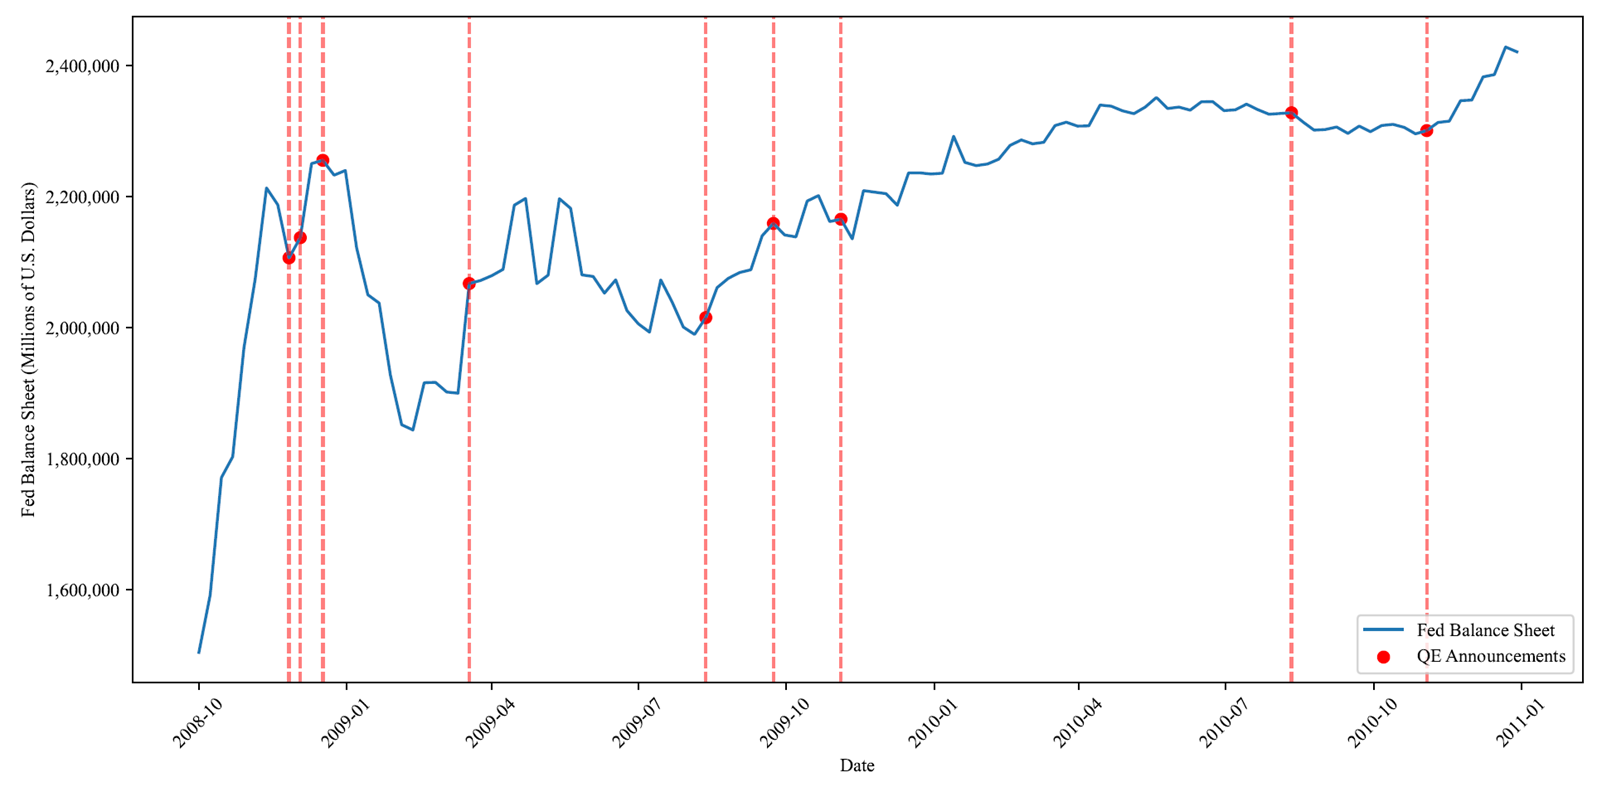
\includegraphics[width=1\linewidth]{Federal Reserve Balance Sheet_LSAP1.png}
    \footnotesize{\textit{Timeline of Federal Reserve Balance Sheet during LSAP 1, Source: FRED Monetary Data}}
\end{figure}

The introduction of LSAP 2 in November 2010 focused on expanding the purchase program to include treasuries. The FOMC made the formal announcement on November 3rd with the intention to purchase a further \$600 billion of long-term Treasury securities by the end of the second quarter of 2011, at a pace of \$75 billion per month. Less than a year later in September of 2011 the FOMC made the reintroduction of Operation Twist for the first time since 1961. The policy involved selling \$400 billion in short-term Treasuries in exchange for the same amount of longer-term bonds, starting in October 2011 and ending in June 2012. The idea was that "by purchasing 400 billion USD worth of Treasury bonds with maturities of 6–30 years and selling bonds with maturities of less than 3 years, the FOMC intended to extend the average maturity of the Fed’s portfolio" (Krishamurthy et al., 2011, p. 337).

Not long after LSAP 3 was introduced in September of 2012. LSAP 3 targeted MBS once again similar to LSAP 2 and was focused on "monthly purchase of \$85 billion through the purchase of mortgage-backed securities (\$40 billion) and longer-term Treasury securities (\$45 billion)" (Krishamurthy et al., 2011, p. 337). The FOMC cited the slow growth in employment and elevated unemployment rate in late 2012 as the driving force behind the decision to implement LSAP 3. The central bank later announced the tapering of LSAP 3 in December 2013 whereby it would lower its monthly long-term Treasury bond purchases to \$40 billion and mortgage-backed securities to \$35 billion a month, both reductions of \$5 billion. In September of 2014, the FOMC published its \href{https://www.federalreserve.gov/monetarypolicy/files/fomc_policynormalization.pdf}{Policy Normalization Principles and Plans}, in which the Committee laid out its plans to reduce its holdings in a gradual and predictable manner primarily by ceasing to reinvest repayments of principal on securities held in the System Open Market Account (SOMA). The SOMA account is used by the Federal Reserve to conduct open market operations.

By far the largest program in nominal dollars the Federal Reserve introduced was in March 2020 (as seen in Figure 3) in response to the COVID-19 induced economic lock downs. On March 15th the FOMC announced the intent to purchase \$500 billion of long-term treasuries and \$200 billion of MBS totalling \$750 billion of expected easing. The desk was instructed to complete these purchases with no explicit timeline but rather at a pace appropriate to ensure smooth continuity in the treasury and MBS markets. According to Levin et al. (2022) LSAP 4 was originally aimed at mitigating the lack of liquidity in the MBS and agency debt markets but later shifted into a broader monetary stimulus program. "From mid-March 2020 to the end of March 2022, the FOMC purchased about \$4.6 trillion in Treasuries and agency MBS, funding those purchases through a corresponding increase in bank reserves and overnight reverse repos" (Levin et al., 2022, p.1). The authors also found that the details of LSAP 4 were initially opaque. Shortly after the program's introduction, a swift change was made to allow for an unlimited amount of easing to support market stability. On March 23, 2024, one week after the initial introduction of LSAP 4, the FOMC instructed the SOMA desk to conduct operations without quantity limits, including the purchase of commercial agency MBS, to ensure the smooth continuity of markets. No explicit pace or timeline was mentioned. The pace in the initial months of the program eclipsed LSAP 3 as "over the four weeks from 18 March to 15 April 2020, the SOMA expanded its holdings of agency MBS by about \$225 billion and its holdings of Treasury notes and bonds by about \$1.3 trillion. In effect, the Fed’s securities purchases within that four-week period were nearly as large as the total amount of purchases made during QE3 in 2012-14" (Levin et al., 2022, p. 7).

While the amounts and timelines of the latter QE programs differed from those during the Great Financial Crisis, the pace of tapering by the FOMC varied significantly between LSAP 4 and LSAP 3. LSAP 4 tapering began in early November of 2021 at pace of \$10 billion in Treasuries and \$5 billion in MBS each month. The tapering in 2021 was double the pace of that seen in LSAP 3 considering also the nominal dollar amount was close to a trillion USD compared to the relatively inconsequential amount of LSAP 3 which can be observed in Figure 2.

\begin{figure}
    \centering
    \captionsetup{justification=centering, labelsep=newline, singlelinecheck=false, font=bf, position=top}
    \caption{Federal Reserve Balance Sheet - LSAP 3 (2012-2014)}
    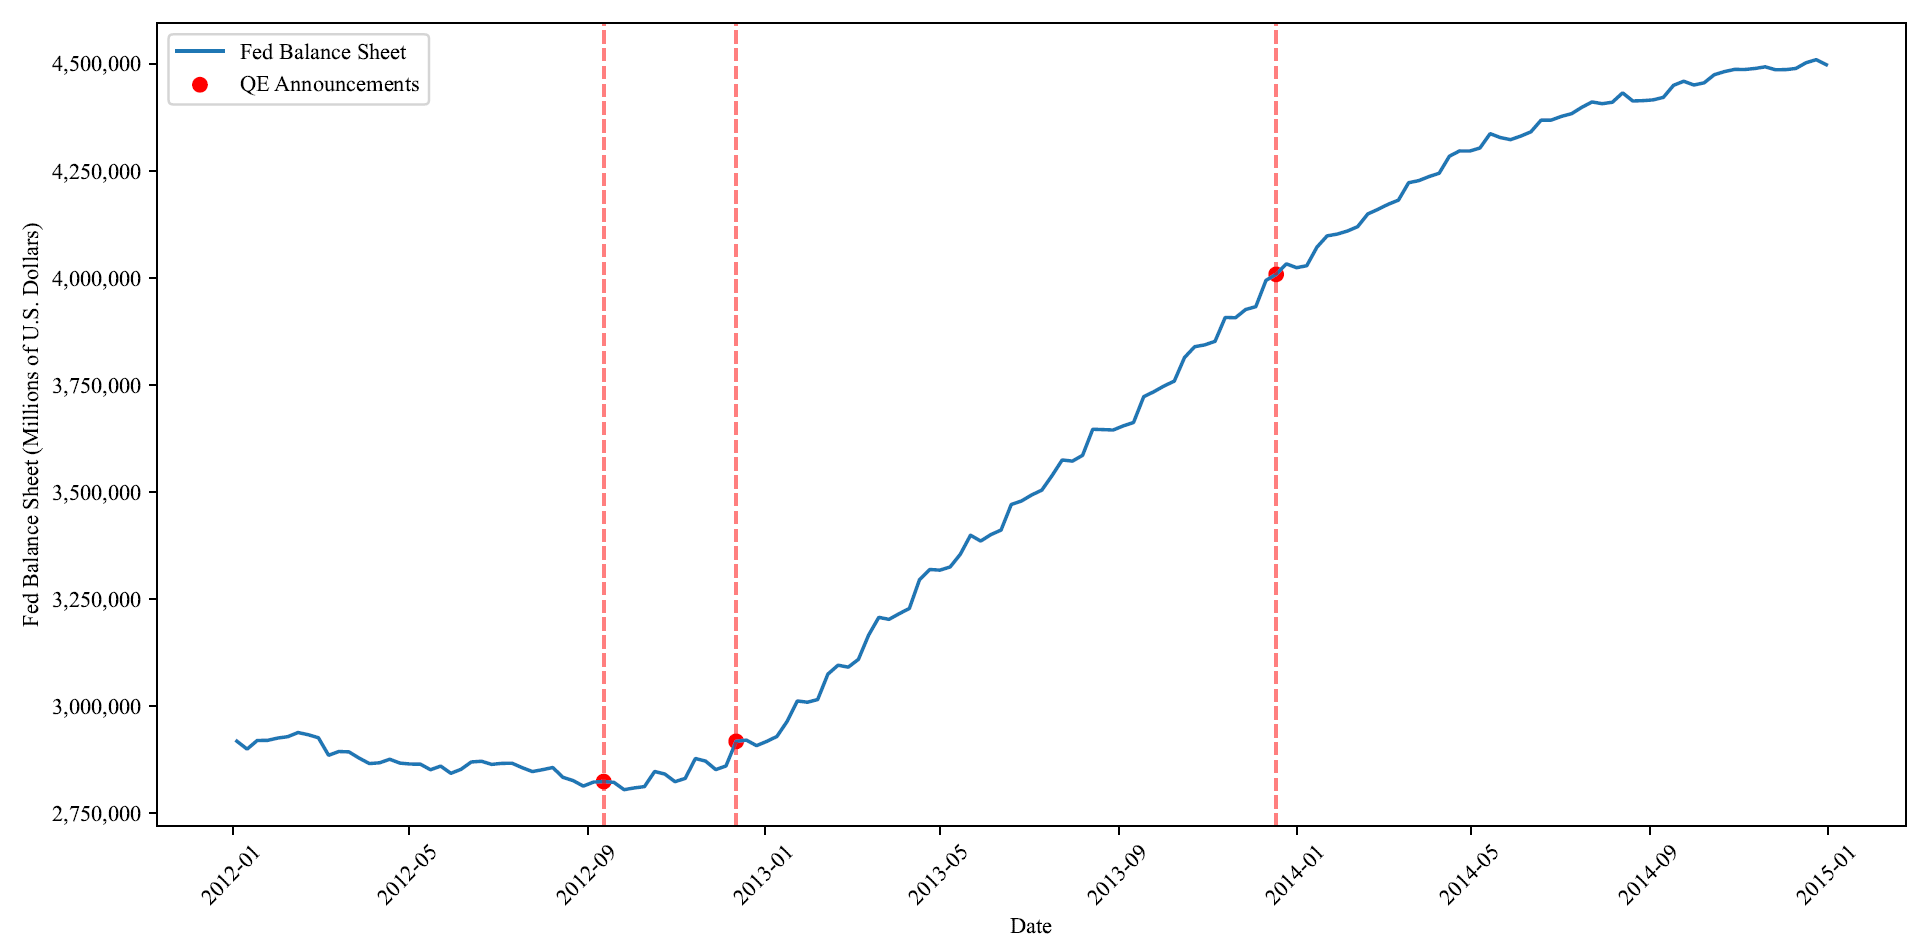
\includegraphics[width=1\linewidth]{Federal Reserve Balance Sheet_LSAP 3.png}
    \footnotesize{\textit{Timeline of Federal Reserve Balance Sheet During LSAP 3, Source: FRED Monetary Data}}
\end{figure}

\begin{figure}
    \centering
    \captionsetup{justification=centering, labelsep=newline, singlelinecheck=false, font=bf, position=top}
    \caption{Federal Reserve Balance Sheet - LSAP 4 (2020-2024)}
    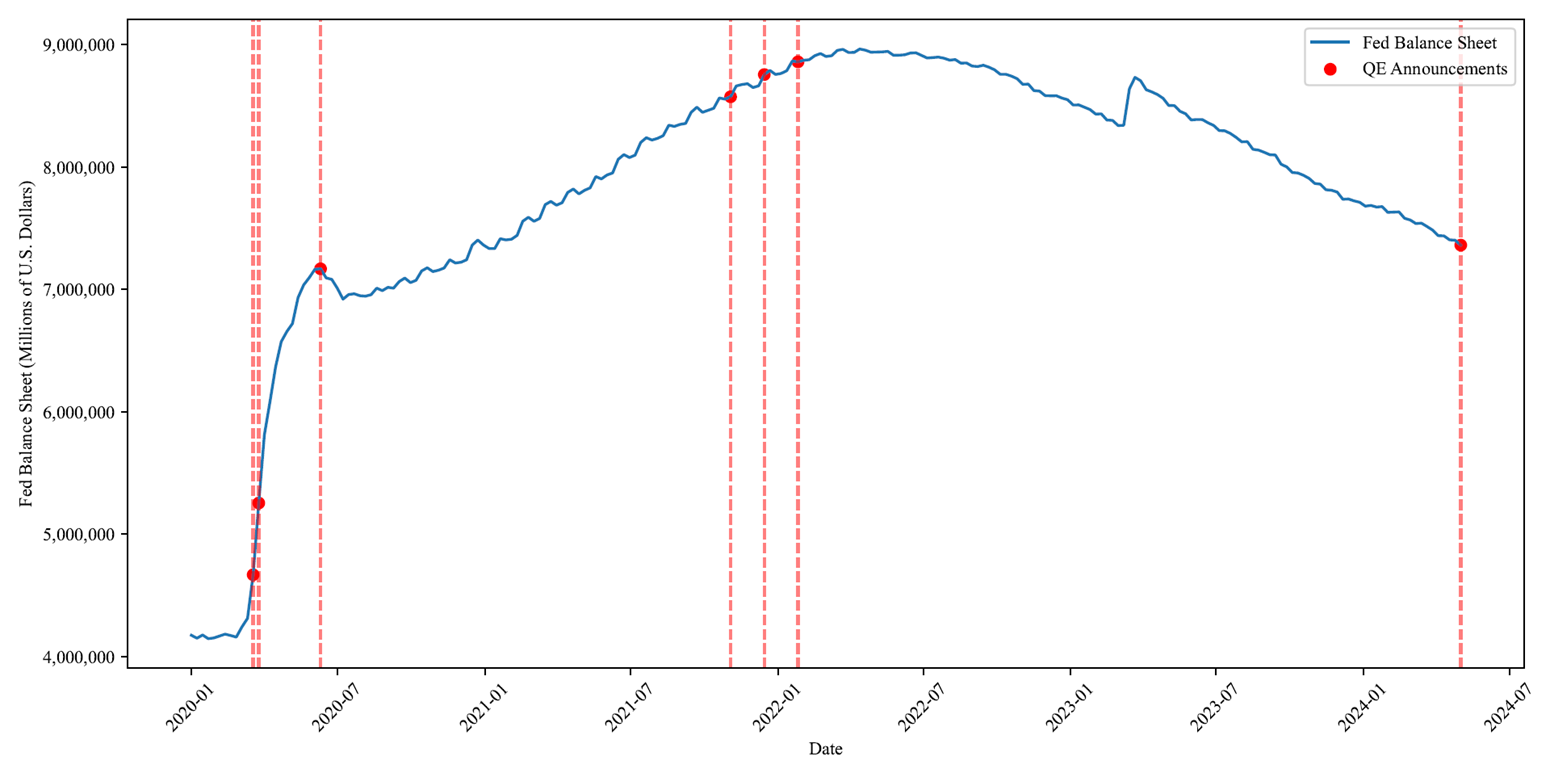
\includegraphics[width=1\linewidth]{Federal Reserve Balance Sheet_LSAP 4.png}
    \footnotesize{\textit{Timeline of Federal Reserve Balance Sheet During LSAP 4, Source: FRED Monetary Data}}
\end{figure}

\begin{table}[H]
\centering
\captionsetup{justification=justified, labelsep=newline, singlelinecheck=false, font=bf}
\caption{Federal Reserve LSAP Programs Overview}
\resizebox{\textwidth}{!}{
\begin{tabular}{l c c c c c}
\toprule
\textbf{Program} & \textbf{Trigger For Intervention}& \textbf{Dates} & \textbf{Securities Purchased} & \textbf{Initial Pace of Purchases (USD)} & \textbf{Total Notional Amount (USD)} \\
\midrule
LSAP 1 & Great Recession & 2008-2010 & Agency Debt, MBS, Long-Term Treasuries & N/A & 1.75 trillion \\
LSAP 2 & Maturity Extension Program & 2010-2011 & Long-Term Treasuries & 75 billion/month & 600 billion \\
LSAP 3 & Housing Market Credit Risk& 2012-2014 & MBS, Long-Term Treasuries & 40 billion/month & N/A\\
LSAP 4 & COVID-19 Pandemic & 2020-2024 & MBS, Long-Term Treasuries, ETFs& 60 billion/month & 2 trillion \\
\bottomrule
\bottomrule
\end{tabular}%
}
\footnotesize{\textit{The Federal Reserve conducted four quantitative easing programs from 2008-2024, the largest in dollar terms was LSAP 4 which was implemented in response to the COVID-19 pandemic.}}
\end{table}

\subsection{Bank of England}
The Bank of England (BoE) followed the Federal Reserve closely in the implementation of QE and was one of the largest programs in proportion to a nation's nominal GDP. The BoE followed the U.S. swiftly in 2009 with the introduction of the first round of QE. In March of 2009 the Monetary Policy Committee (MPC) announced that it would purchase £75 billion of assets over three months funded by central bank reserves, with conventional bonds likely to constitute the majority of purchases. Gilt purchases were to be restricted to bonds with a residual maturity of between 5 and 25 years (Glick and Leduc, 2012).  The MPC later announced the program was to be extended by an additional £50 billion to a total of £125 billion, these purchases were intended to still remain in the scope of long-dated gilts but private sector assets were eventually included. Lyonnett and Werner (2012) find that even prior to the official March 2009 QE announcement the \href{https://www.bankofengland.co.uk/-/media/boe/files/news/2008/april/special-liquidity-scheme}{Special Liquidity Scheme in April 2008} closely resembled conventional quantitative easing whereby financial institutions could swap illiquid assets for short-dated gilts for up to three years. These were considered lending transactions and were not included on the Bank of England's balance sheet and thus could not be considered a monetary expansion. 

The MPC would further expand QE1 two additional times in August 2009 (£50 billion) and again in November of the same year (£25 billion). The Bank cited rising deflation and falling output in 2009 as the driver of the multiple expansions of QE1. The Central Bank would cumulatively purchase £175 billion in assets by the end of October 2009 and would include gilts with a residual maturity extending beyond three years. The MPC would complete QE1 extending the final round of purchases to £200 billion in November 2009. The pace of purchases under QE1 was the fastest until QE5 from the Bank of England at an implied speed of £6bn per week on average, QE2-4 were conducted at roughly half the pace of QE1 (Bussetto et al., 2022).

QE2 was introduced on October 6th 2011 roughly two years after the conclusion of QE1. The program was introduced with the intent to purchase above market expectations of £75 billion in gilts over a four month time frame. No specific mention of maturity of gilt purchases was made and the program was extended once more in February 2012 to increase the total program purchases by an additional £50 billion of gilts. The Bank cited slower economic growth at home and abroad, especially in the UK's main export markets, as well as problems in the euro zone, and strains on the banking system. 

QE3 and QE4 were one time announcements in July of 2012 and August 2016 respectively. In July 2012 soon after the last announcement of QE2 the Bank of England's monetary policy committee voted to raise the total amount of quantitative easing to £375 billion an increase of a further £50 billion of asset purchases. Finally in 2016 proceeding the vote from the U.K. to part from the EU, the MPC decreased its growth forecast and launched a £70bn bond-buying programme. The purchase of up to £10 billion of UK corporate bonds; and an expansion of the asset purchase scheme for UK government bonds of £60 billion. QE4 had a longer-time horizon of 6 months compared to the historical average program timeline of 3-4 months. QE4 was the first program introduced by the MPC that would include corporate debt which had not been purchased in the previous three programs. The decisions from the MPC came after a series of negative economic data in the wake of the vote to leave the European Union in June (Bussetto et al., 2022). The MPC also introduced a new \href{https://www.bankofengland.co.uk/-/media/boe/files/quarterly-bulletin/2018/term-funding-scheme-web-version.pdf}{Term Funding Scheme}, up to £100 billion funded from newly-printed money to ensure the pass through of the subsequent rate cut onto businesses and consumers.

The Central Bank's most recent QE program would follow the Federal Reserve's actions in the wake of the COVID-19 pandemic. Three distinct QE5 announcements were made in 2020 followed by two intentions to taper the program in early and late 2022. In March 2020 the MPC announced the intent to increase the bank's holdings of bonds by £200 billion, financed by printing money. Later in June the total asset purchases were to be increased by £100 billion to further aid the recovery. Finally in November of that same year the MPC would announce the intent to purchase a final additional round of £150 of gilts amid the second European COVID-19 lockdown.

The MPC would provide few detail at their February meeting in 2022 about the intended taper of QE5. The explicit announcement of the taper would come later in the year in September. The MPC voted unanimously to reduce the stock of purchased gilts, financed by the issuance of central bank reserves, by £80 billion over the next twelve months, to a total of £758 billion, in line with the strategy set out in the minutes of the August meeting.

\subsection{European Central Bank}

The European Central Bank (ECB) formally began quantitative easing in early 2015 with the introduction of the Asset Purchase Programme. Prior to this the monetary authority purchased covered bonds under the Securities Market Programme (SMP) which was not explicitly defined as quantitative easing. While the SMP was primarily used to bolster market liquidity during the euro-zone Sovereign Debt Crisis that began in 2010 the program was in fact reflective of early quantitative actions by the ECB (Smith, 2020).

According to Smith (2020) SMP was introduced due to the lack of demand for Sovereign Debt from euro-zone nations such as Spain, Italy and Greece. The program details were announced by the ECB on March 10, 2010 and was concluded on September 6, 2012 and was replaced by the Outright Monetary Transactions (OMT) program. At that time, purchases made under the SMP totaled €218 billion. The program which was considered a surprise by market participants had two formal announcements to the public, one on March 10, 2010\footnote{Smith (2020) details that the exact start date of the SMP is unclear amongst the literature. The program was announced on May 9, with details released on May 10. The official legal decision, signed on May 14, states that the program took effect the day after its publication on the European Central Bank (ECB) website.} which detailed the program without explicit mention of the timeline and the second on August 7, 2011 detailing a reactivation an expansion which included Italy and Spain in the sovereign debt purchases.  

While there was formal announcement of the program there was no explicit mention of the key features such as the targeted securities, maturities , amount or timeline intended by the ECB. After the conclusion of the program it was reported that over half of the securities purchased under the SMP were Italian government bonds, roughly €102.8 billion (nominal).

Cour-Thimann and Winkler (2013) explain the difference between direct monetary stimulus, such as quantitative easing, and the 'non-standard' measures introduced by the ECB in 2011. The authors describe these measures as complementary to standard interest rate decisions, aimed at supporting the effective transmission of monetary policy to the economy rather than providing additional direct monetary stimulus. They note that while typical quantitative easing programs, like those in the U.S. and U.K. during the Great Recession, resulted in central bank balance sheets increasing by over 150\%, the ECB's balance sheet grew by only 50\%. Despite the smaller increase, the ECB still conducted open market purchases of €40 billion in euro-zone covered bonds after the conclusion of the Securities Markets Programme (SMP) in late 2011. The scale of balance sheet expansion does not change the nature of the intervention. Both involve large-scale asset purchases aimed at increasing liquidity and stimulating the economy. The ECB's focus on lending against collateral rather than purchasing assets outright is cited as a distinguishing factor. However, the purchase of €40 billion in euro-zone covered bonds after the SMP's conclusion still represents direct market intervention similar to QE. The effect of such purchases on market liquidity and asset prices aligns with conventional QE objectives. 

In October 2014, the ECB formally discussed QE, agreeing on the details of a program for purchasing Asset-Backed Securities and Covered Bonds, known as the Asset Purchase Programme. On January 22, 2015, the ECB formally announced it would purchase securities at a pace of €60 billion per month until at least September 2016. This was the first time the ECB had announced a purchase program with an explicit amount, pace, and timeline. The goal was to continue the program until the Governing Council observed a sustained adjustment in the path of inflation consistent with achieving rates below, but close to, 2\% over the medium term. The ECB would buy bonds issued by euro area central governments, agencies, and European institutions in the secondary market using central bank money, which the selling institutions could then use to buy other assets and extend credit to the real economy. This approach aimed to ease financial conditions. The APP concluded in December of 2018 after three years of security purchases. The program resumed in 2020 following the global closures as a result of the COVID-19 pandemic. 

\begin{table}[H]
\centering
\captionsetup{justification=justified, labelsep=newline, singlelinecheck=false, font=bf}
\caption{Net Purchases under the APP by the European Central Bank (2015-2018)}
\begin{tabularx}{\textwidth}{l C}
\toprule
\textbf{Period} & \textbf{Net Purchases (€)} \\
\midrule
03/2015 to 03/2016 & 60 billion \\
04/2016 to 03/2017 & 80 billion \\
03/2017 to 12/2017 & 60 billion \\
01/2018 to 09/2018 & 30 billion \\
10/2018 to 12/2018 & 15 billion \\
\bottomrule
\bottomrule
\end{tabularx}
\footnotesize{\textit{The European Central Bank implemented the Asset Purchase Programme from 2015-2018 purchasing a total of €245 of assets. Source: ECB (2024)}}
\end{table}

Three days after the announcement of LSAP 4 by the Federal Reserve on March 18, 2020, the European Central Bank introduced the Pandemic Emergency Purchase Programme (PEPP) with a total of €750 billion in purchases. The program included any assets available under the existing asset purchase programme (APP). The PEPP was increased twice more in 2020: by €600 billion in June and €500 billion in December. On December 16, 2021, the Governing Council announced that purchases under the PEPP would be discontinued, signaling the intent to taper the program.

\section{Quantitative Easing and its Transmission Channels to Oil Markets}

\subsection{Foreign Exchange}
The foreign exchange channel affects oil prices through the devaluation or appreciation of a countries currency from an expansion in long term rates through quantitative easing. The expectation is that if a central bank announces the intention to increase the scale of open market purchases all else equal the country's currency would depreciate against foreign partners.

Frankel (2006) discusses the implications of currency fluctuations as it related to oil prices, the author dictates that monetary policy tightening appreciates a currency against the dollar preventing the domestic price of oil from rising. Due to global oil futures being priced in U.S. dollars any monetary policy conducted by the Federal Reserve will have an impact on the spot value of the U.S. dollar thus affecting oil prices (Rosa, 2014). Rosa finds that upon observing oil movements on days where there is an LSAP Surprise the exchange rate channel cannot explain all the variation in the price of the front-month WTI futures. The author tests the hypothesis of the exchange rate channel by observing the intraday percentage change in the dollar price of crude oil from 10-min before to 50-min after the FOMC LSAP announcement, and the intraday percentage change in the U.S. dollar exchange rate against five currencies (the euro, the British pound, the Canadian dollar, the Swiss franc, and the Japanese yen). 

\begin{figure}
    \centering
    \captionsetup{justification=centering, labelsep=newline, singlelinecheck=false, font=bf, position=top}
    \caption{Brent Crude Front-Month Futures Contract and EUR/USD Exchange Rate Correlation (2008-2024)}
    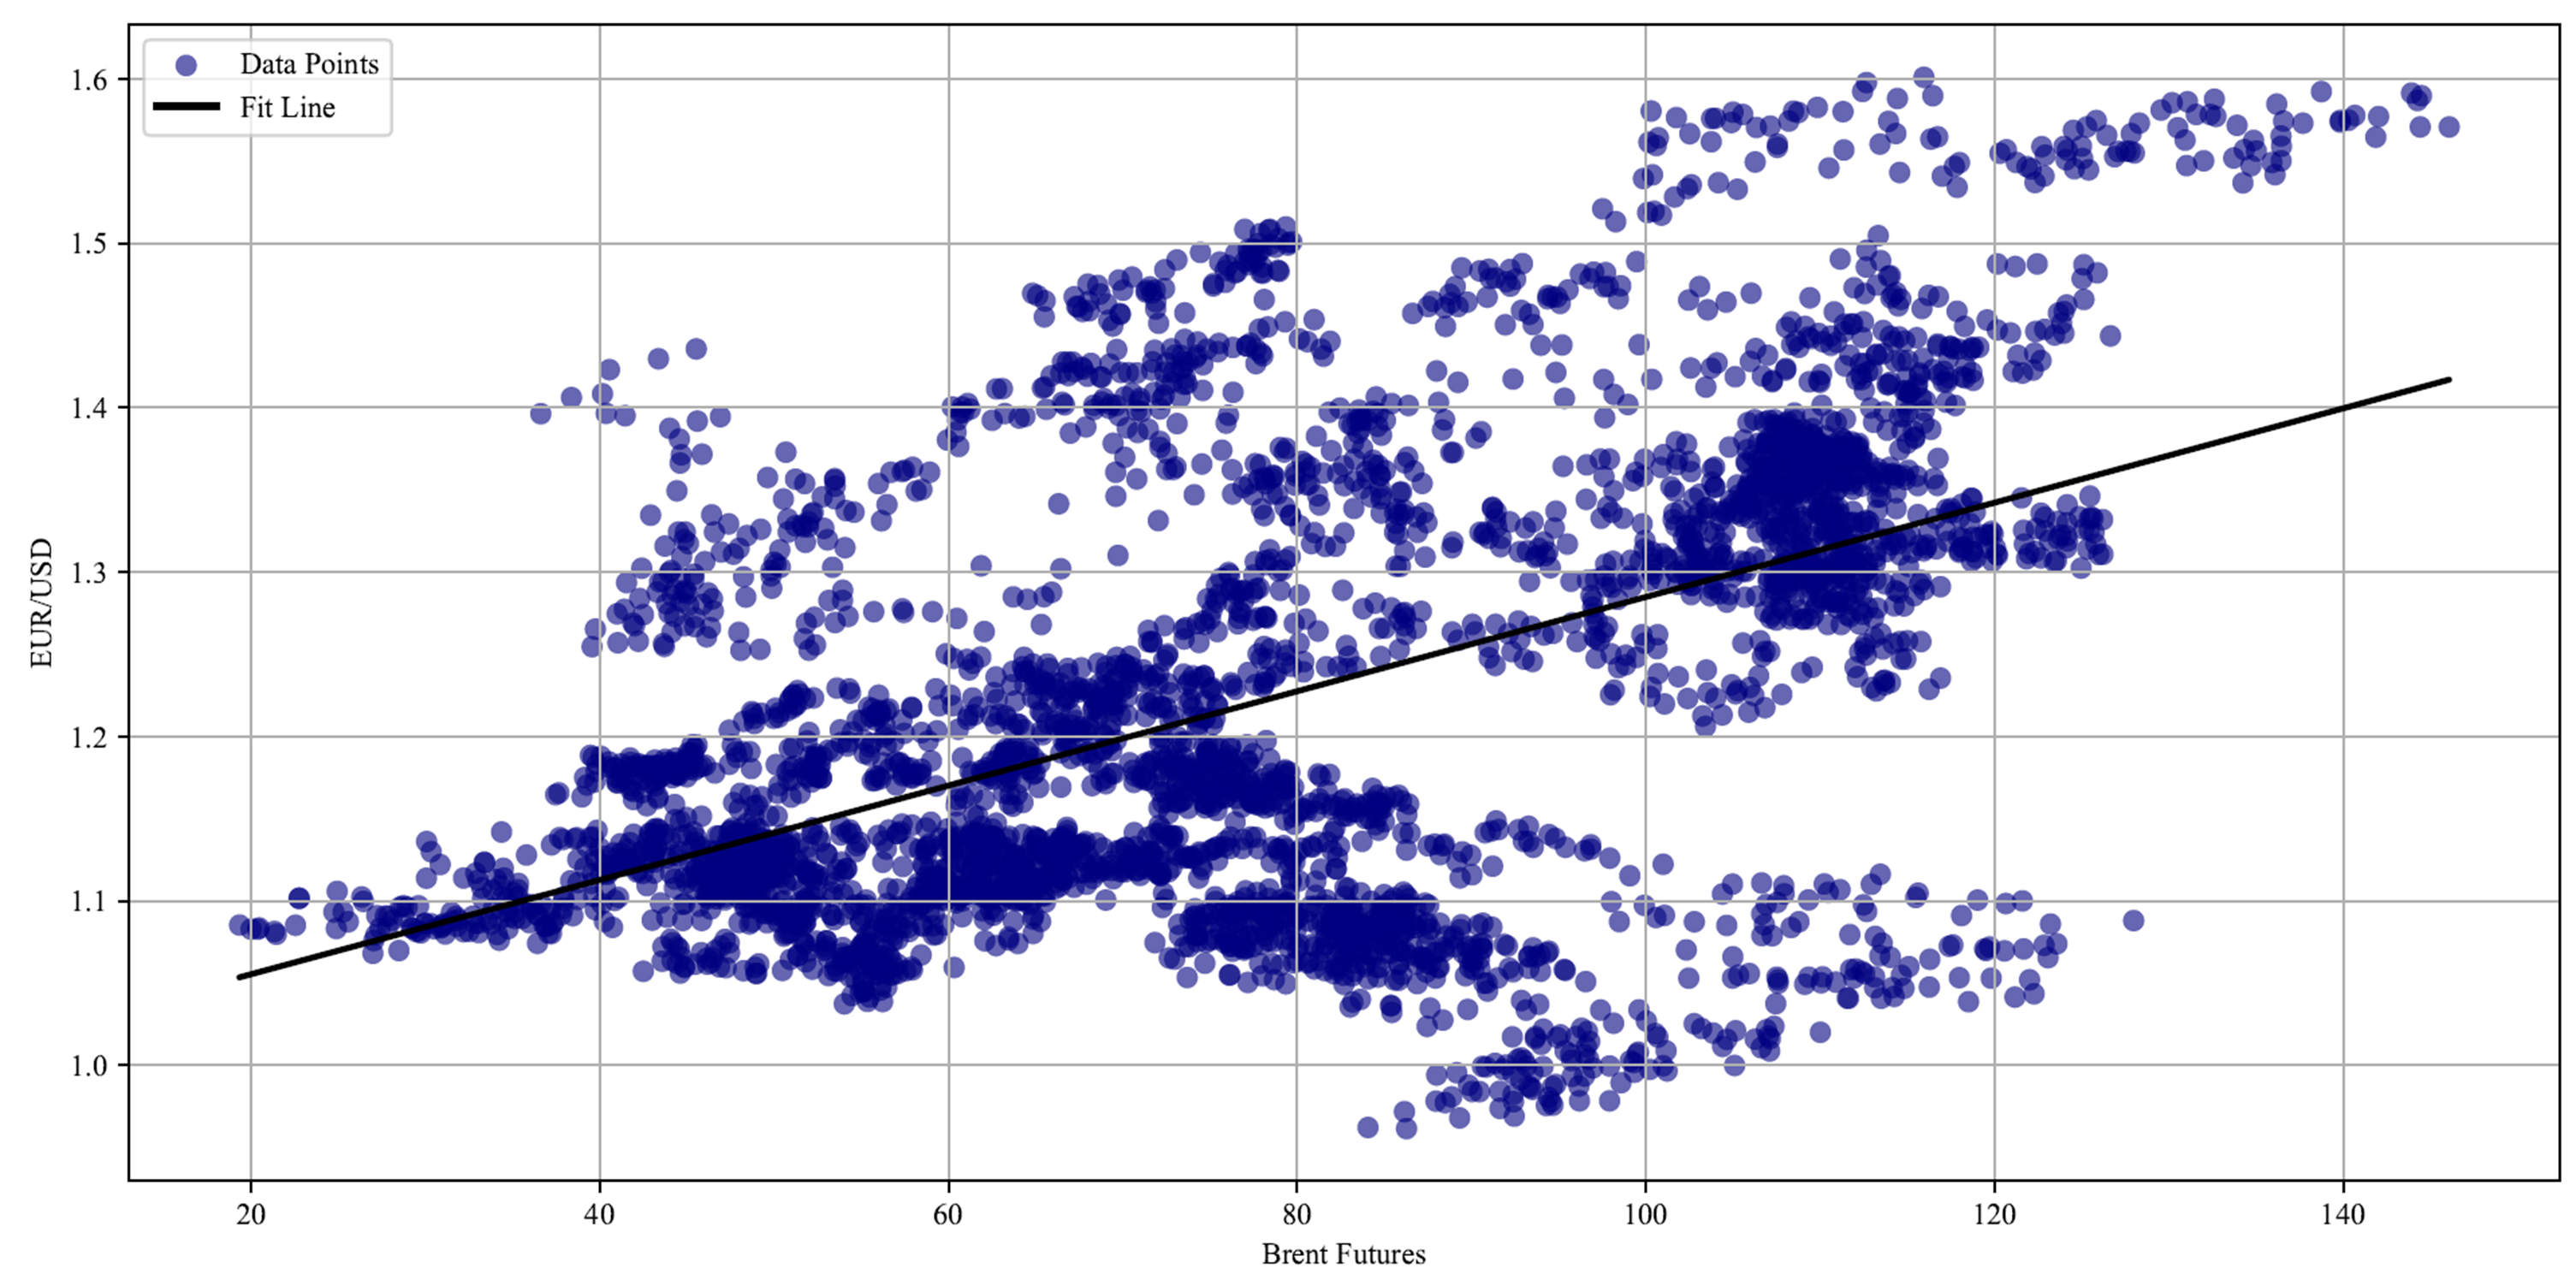
\includegraphics[width=1\linewidth]{Brent Crude_EUR-USD.png}
    \footnotesize{\textit{Brent Crude Front-Month Futures Contract and EUR/USD Exchange Rate from the Great Recession to COVID-19, Source: Bloomberg}}
\end{figure}

\begin{figure}
    \centering
    \captionsetup{justification=centering, labelsep=newline, singlelinecheck=false, font=bf, position=top}
    \caption{Brent Crude Front-Month Futures Contract and EUR/USD Exchange Rate Correlation Sample (2008/11/01 - 2008/12/30)}
    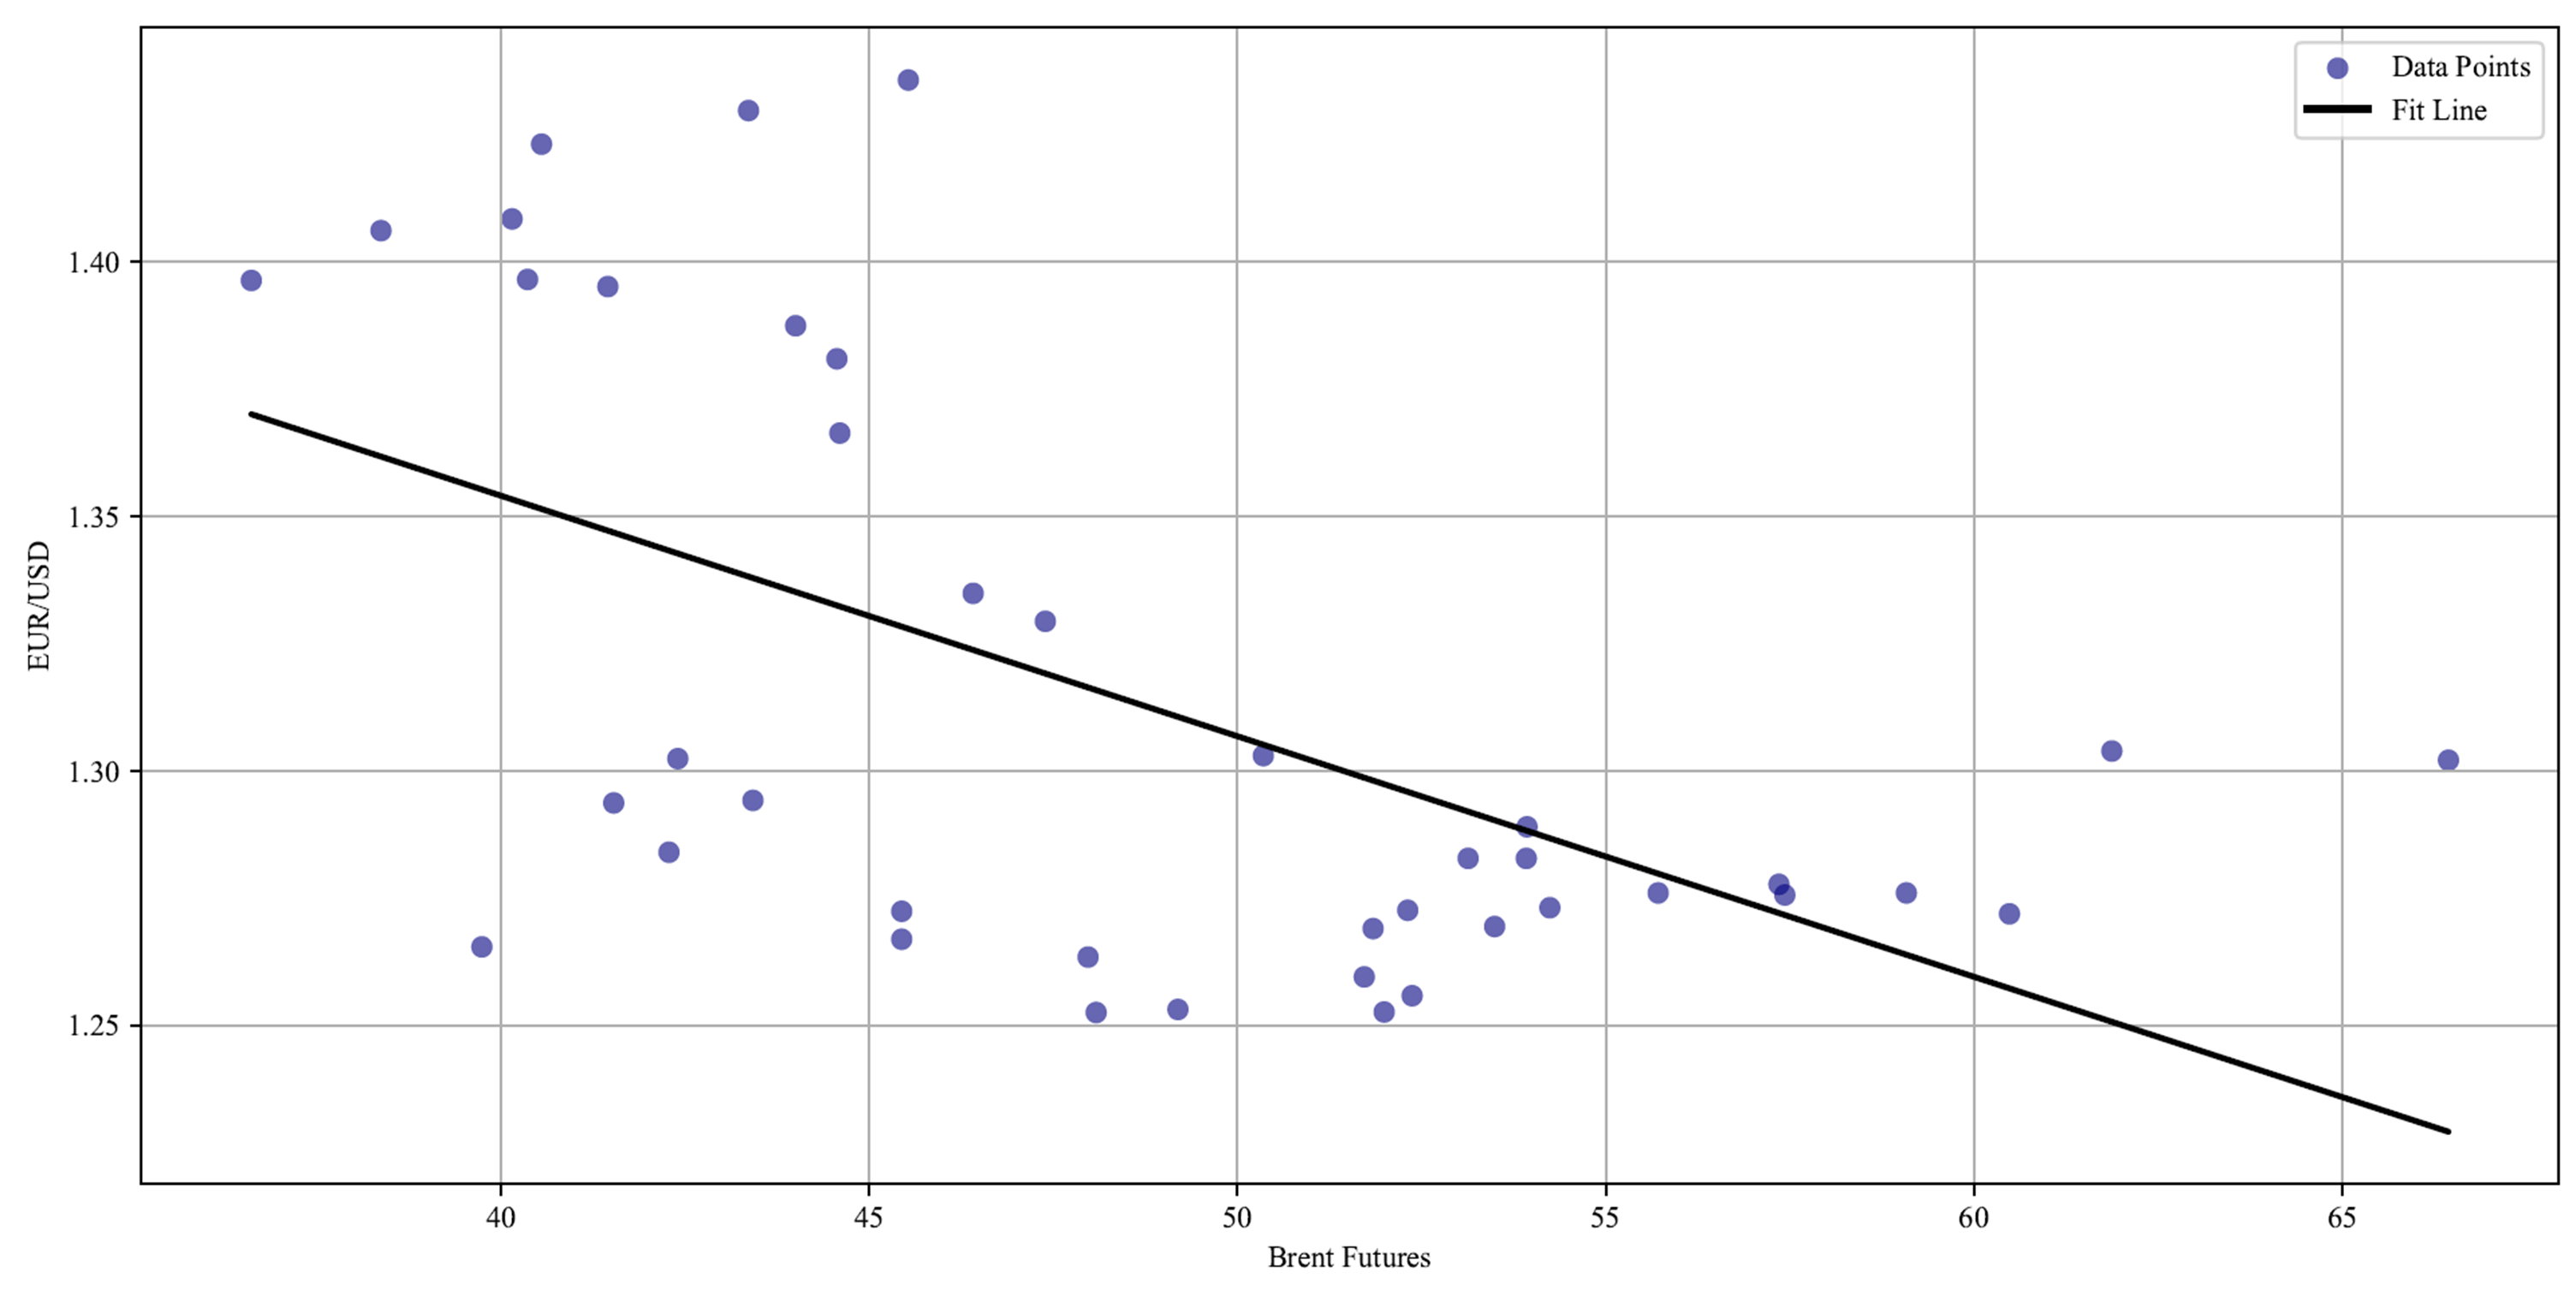
\includegraphics[width=1\linewidth]{Brent Crude_EUR-USD Sample.png}
    \footnotesize{\textit{Brent Crude Front-Month Futures Contract and EUR/USD Exchange Rate during initial months of LSAP 1 Announcements made by the Federal Reserve, Source: Bloomberg}}
\end{figure}

A mechanical exchange rate channel would imply that the exchange rate perhaps USD/EUR would exactly offset the change in price of oil specifically WTI with respect to a FOMC LSAP announcements. Figure 4 plots the correlation of Brent Crude Front-Month Futures and the EUR/USD exchange rate. Since the introduction of QE across major central banks in 2008 both Brent Crude futures and the EUR/USD have exhibited a positive correlation meaning a depreciation in the USD in which major oil benchmarks are priced in makes the contract relatively cheaper for foreign buyers increasing buying activity. Figure 5 plots a sample of Figure 4 data during the three initial announcements of LSAP 1 by the Federal Reserve. The correlation during the two months of the introduction of LSAP 1 was predominantly negative. Miranda-Pinto et al. (2023) hypothesize that all else equal an appreciation of the USD dollar increases the price of commodities in foreign local currency, which then decreases demand and stimulates supply, thus, putting downward pressure on prices. The authors observe that most commodity prices overshoot with respect to the change in the exchange rate in response to U.S. monetary tightening. Soriano and Torro (2022) more recently study the effect of ECB monetary policy announcements and their effect on high-frequency Brent Crude futures prices dating back to the great recession. The authors results show that the pass-through of monetary policy to the oil Brent price is mostly due to the exchange rate response on event days. Brent Crude futures are priced in USD therefore the natural channel one could hypothesize as having a significant pass through to foreign oil prices would be the change in the USD/EUR. 

Glick and Leduc (2012) observe various great recession period LSAP announcements and their effect on foreign exchange performance. The results for the Bank of England LSAP announcements and their daily effect on the Dollar/GBP movement is quite insignificant for a surprise quantitative easing announcement. The authors find the contrary movement for U.S. Federal Reserve announcements as all observed currency pairs were statistically significant for both LSAP positive and negative surprises. 

\subsection{Economic Expectation}
The economic expectation channel affects oil futures through the expectation of future economic growth. The general hypothesis of the channel is that if the market expects future economic growth to be positive this would benefit oil futures. Yang et al. (2022) test this channel through GDP expectation as in Jarociński and Karadi (2020) and its effects on oil prices. The unexpected increase in the interest rate can make some market participants more optimistic about future economic growth, empirical results prove that GDP expectation is one of the channels through which central bank information and monetary policy shocks can affect oil prices. Contrary to how market participants may expect that a positive LSAP announcement would depress long-term rates and feed through to commodities, the economic expectation channel passes through in the opposite way. If the central bank announces the intent to taper an existing quantitative easing program this would send positive signals about future economic growth thus potentially lowering inflation expectations and boosting oil futures through the expectation of economic stability.

\subsection{Finance/Investor Displacement}
This section deals with observing investor displacement that occurs in the asset markets where central banks will direct their action towards such as agency debt, mortgage backed securities or other securitized assets as part of their LSAP programs. Glick and Leduc (2012) discuss this channel they call 'portfolio balance effects' whereby the expectation of central bank purchases reduces the overall supply of longer-term securities available to market participants. The authors discern that "If some investors, such as pension funds or insurance companies, have a preference to hold longer-term securities, these 'habitat' preferences make the yields on securities of different maturities partly depend on their relative supplies. As a result, central bank purchases that reduce the stock of long term securities held by the private sector push up the price of these securities, lessen the term premium required to compensate investors to hold them, and hence lower long-term interest rates" (Glick and Leduc, 2012, p. 2080).   Rosa (2014) also examines the finance channel in witch the author refers to as 'portfolio balance' whereby the LSAP programs conducted by the Federal Reserve displaces private investors from the treasury and mortgage backed security market and moves money to other assets classes one of those being commodities.

Figure 6 and 7 plot the Commercial and Non-Commercial change in WTI future open interest surrounding Federal Reserve LSAP announcements. Across both figures data shows that the variability in open interest is much smaller for tightening announcements compared to those of easing. Furthermore as observed in the boxplots, the median change in open interest for non-commercial traders in WTI futures is positive during tightening and negative during easing, reflecting speculative responses to monetary policy signals. Non-commercial traders, such as hedge funds, may increase positions during tightening due to expectations of economic strength and higher oil demand, while reducing positions during easing due to concerns about economic weakness. Conversely, commercial traders, who use futures for hedging, show opposite behavior. They may decrease open interest during tightening due to higher costs and risks, while increasing it during easing as they anticipate stronger economic activity and seek to manage risks by locking in prices. This divergence highlights how speculative and hedging motives drive different reactions to monetary policy changes.

\begin{figure}
    \centering
    \captionsetup{justification=centering, labelsep=newline, singlelinecheck=false, font=bf, position=top}
    \caption{Impact of Federal Reserve LSAP Announcements on Commercial Open Interest Changes in WTI Front-Month Futures}
    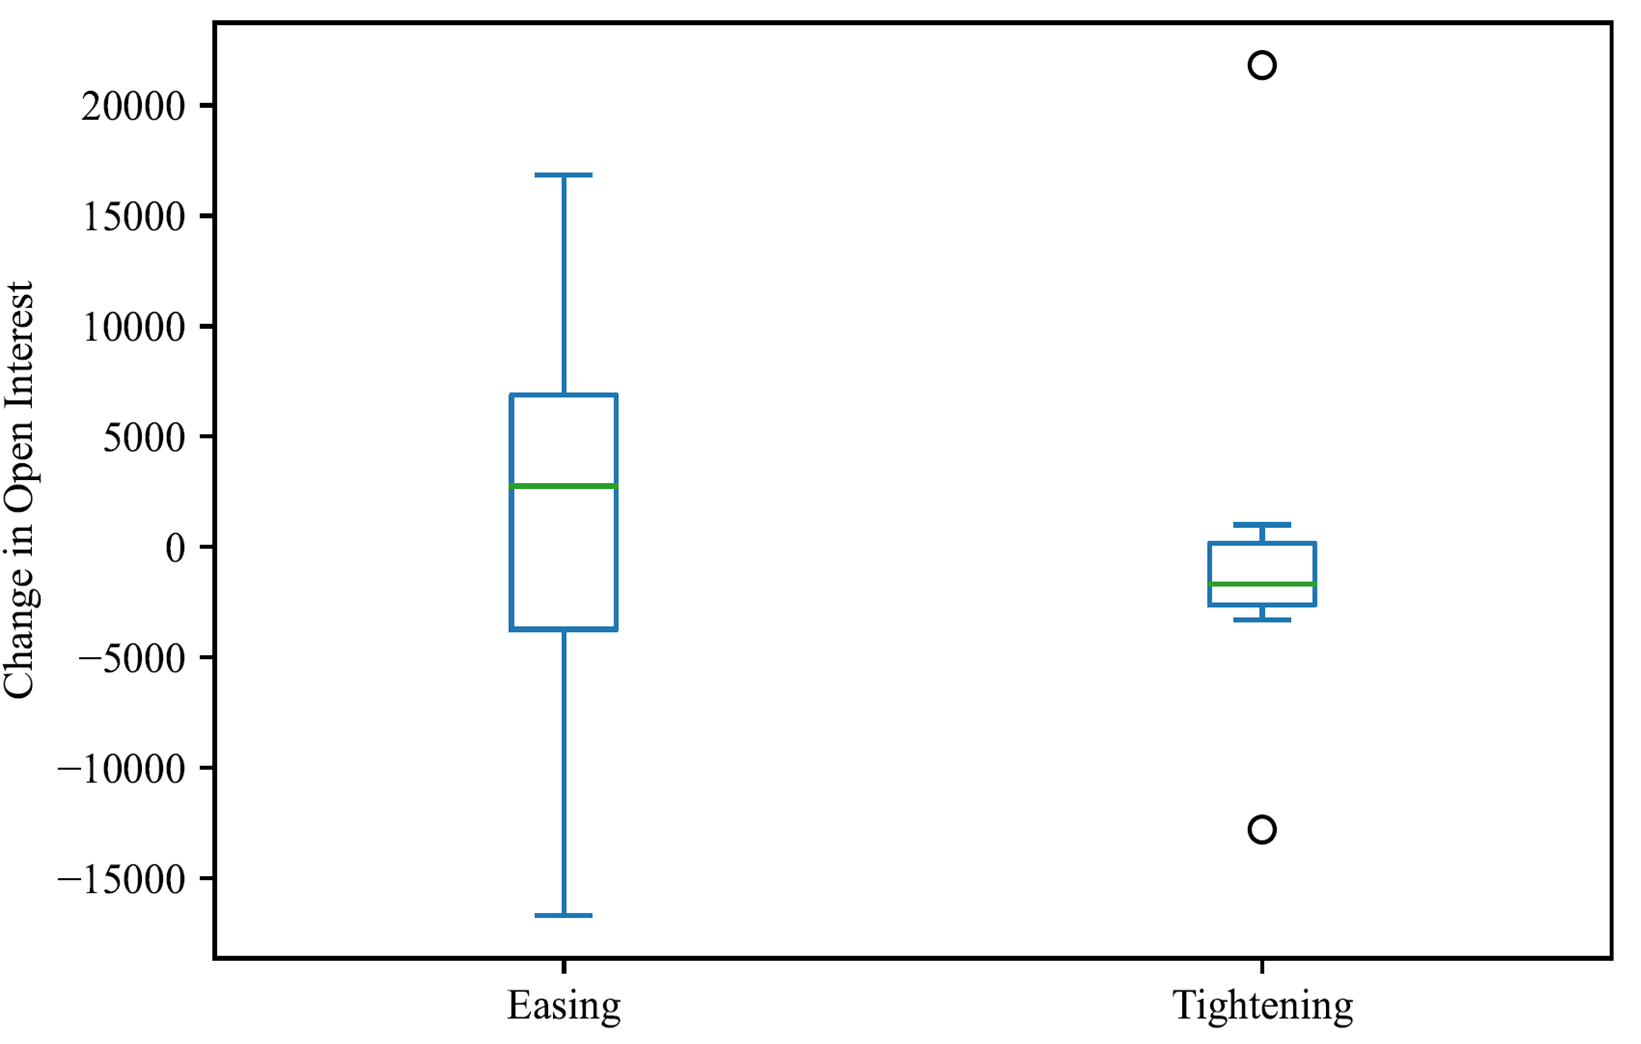
\includegraphics[width=1\linewidth]{WTI_Open Interest_Comm.png}
    \footnotesize{\textit{Commercial Open Interest: This represents the positions held by commercial entities, such as producers, consumers, or other businesses that use the futures contracts to hedge against price fluctuations. The green line represents the median value. The top and bottom lines of the box show the maximum and minimum values, respectively, while the edges of the box represent the first and third quartiles (Q1 and Q3). Dots represent outliers in the data. Source: CFTC Legacy Report}}
\end{figure}


\begin{figure}
    \centering
    \captionsetup{justification=centering, labelsep=newline, singlelinecheck=false, font=bf, position=top}
    \caption{Impact of Federal Reserve LSAP Announcements on Non-Commercial Open Interest Changes in WTI Front-Month Futures}
    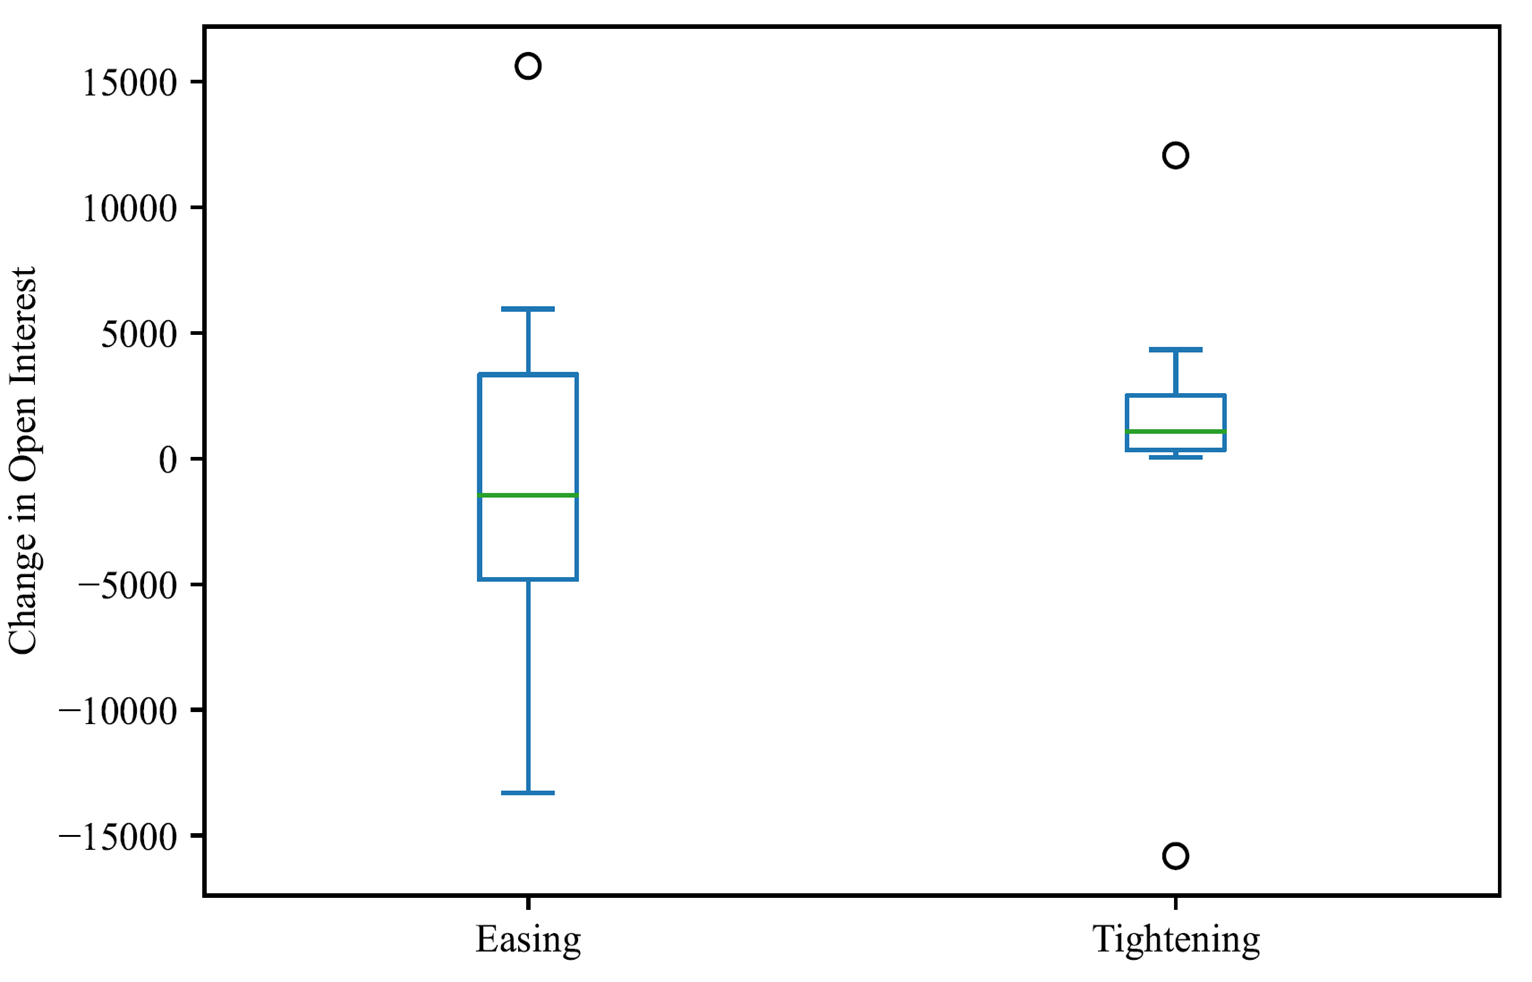
\includegraphics[width=1\linewidth]{WTI_Open Interest_NonComm.png}
    \footnotesize{\textit{Non-Commercial: This refers to positions held by speculative traders, such as hedge funds and individual investors, who are not directly involved in the physical market. These traders typically use futures contracts to speculate on price movements rather than to hedge.
    The plot circles indicate outliers. The green line represents the median value. The top and bottom lines of the box show the maximum and minimum values, respectively, while the edges of the box represent the first and third quartiles (Q1 and Q3). Dots represent outliers in the data. Source: CFTC Legacy Report}}
\end{figure}


\subsection{Inventory}
The inventory channel interacts with quantitative easing (QE) and quantitative tightening (QT) primarily through changes in borrowing rates. When both short- and long-term rates respond to a central bank's Large-Scale Asset Purchase (LSAP) announcement, the opportunity cost of holding physical inventory in the oil market is affected.

For instance, when a central bank announces the tapering of an LSAP program, long-term rates are expected to rise, increasing the cost of carrying physical commodities. This increase can lead to lower inventories, higher supply, and, consequently, lower oil prices.

Quantitative easing can reduce the cost of carrying physical commodities like oil by lowering financing and storage costs. As a result, the commodity's convenience yield may decrease because holding physical inventories becomes relatively less valuable compared to financial assets. Under QE conditions, the perception of scarcity or immediate demand for physical commodities may diminish.

Conversely, under quantitative tightening announcements made by central banks, the convenience yield is likely to increase due to the higher carrying costs of commodities. The increase in the convenience yield can be attributed to higher financing costs, which reduce the incentive to hold physical oil inventories. Consequently, the premium (convenience yield) associated with holding physical oil increases.

\subsection{Summary of Channel Hypotheses}
The hypotheses for each channel and their relationship with oil futures are outlined below. The indicator variables used will be discussed in Section 6.

\begin{longtable}{p{0.10\textwidth} p{0.55\textwidth} p{0.10\textwidth} c}
    \captionsetup{justification=justified, labelsep=newline, singlelinecheck=false, font=bf}
    \caption{Hypotheses: Monetary Policy Channels and Their Impact on Oil Prices} \\ % Add your title here
    \toprule
    \textbf{Channel} & \textbf{Hypothesis} & \textbf{Variable} & \textbf{Relationship} \\
    \midrule
    \endfirsthead
    \toprule
    \textbf{Channel} & \textbf{Hypothesis} & \textbf{Variable} & \textbf{Relationship} \\
    \midrule
    \endhead
    Foreign Exchange & Benchmark oil futures are priced in U.S. dollars. According to theory, QE announcements are expected to devalue the U.S. dollar against foreign currencies, thus potentially boosting oil futures. & Exchange Rates & - \\
    \addlinespace
    Economic Expectation & QE influences market expectations regarding future economic growth. Unexpected QE announcements can alter oil demand forecasts, thereby affecting oil prices. & Break-even Inflation & - \\
    \addlinespace
    Inventory & QE affects oil prices by altering the opportunity cost of holding physical inventory. A decrease in long-term rates due to QE can lower the cost of carrying inventory, potentially reducing supply and boosting oil prices. & EIA Oil Stock & + \\
    \addlinespace
    Finance & Displacement of investors from MBS or treasury markets due to QE could redirect capital towards commodities in pursuit of higher returns. Monitoring Commitment of Trader Reports (COT) could reveal evidence of this re-balancing. & COT-Report Open Interest & + \\
    \bottomrule
    \bottomrule
\end{longtable}

\section{Data}

\subsection{Data on Large-Scale Asset Purchase Program Announcements}
LSAP announcement dates adhere to definitions outlined in Rosa (2014), Wright (2011), Glick and Leduc (2012), and are cross-referenced with the \href{https://www.ft.com/bankaction}{Financial Times 'Bond buying and easy money: a timeline of central bank action'}. Additionally, any explicit mentions of large-scale asset purchases by the Federal Reserve, European Central Bank, or Bank of England are included. In instances where an LSAP announcement falls on a weekend, the data for the subsequent Monday is used as the return for the variables. 

For the 20 announcements made by the Federal Reserve that pertained to either a material mention of quantitative easing or tightening, from 2008-2024 only one announcement was called on a weekend (March 15th, 2020) during the beginning of economic closures as a result of the COVID-19 pandemic. This announcement marked the beginning of  LSAP 4 from the Federal Reserve with the intent to purchase \$500 billion of treasury securities and \$200 billion of MBS. The European Central Bank announcement set encompasses 16 quantitative easing related announcements with the explicit date being sourced from the press releases from the European Central Bank news release database. From 2010-2023 of the 16 announcements the majority were released on either Wednesday or Thursday of the business week aside from the August 7th 2011 announcement which was made on a Sunday. This announcement was made to alter the Securities Market Programme to include sovering debt from Italy and Spain. Finally the Bank of England announcement data set is sourced primarily from Glick and Leduc (2012) as well as the \href{https://www.ft.com/bankaction}{Financial Times 'Bond buying and easy money: a timeline of central bank action'}. All 13 identified announcements from the Bank of England from 2009-2022 occurred on a Thursday.

In identifying and examining quantitative easing (QE) and quantitative tightening (QT) announcements, three distinct categories can be delineated within the dataset: 

\begin{enumerate}
    \item \textbf{Explicit QE Announcements:} These include announcements that explicitly state the intent to conduct quantitative easing or expand an ongoing large-scale asset purchase program. For example, on November 3rd, 2010, the Federal Reserve announced its intent to purchase \$600 billion of longer-term Treasury securities at a pace of \$75 billion per month.
    
    \item \textbf{Explicit QT Announcements:} These refer to announcements that explicitly mention the intent to conduct quantitative tightening or taper the purchases of an ongoing large-scale asset purchase program. For instance, on December 15th, 2021, the Federal Reserve announced it would double its speed of tapering, reducing its bond purchases by \$20 billion in Treasuries and \$10 billion in mortgage-backed securities each month.
     
    \item \textbf{Implicit QE/QT Announcements:} This category includes announcements that implicitly refer to quantitative easing or tightening without explicitly stating it. These announcements may involve language indicating the central bank's intention to support financial markets or the economy through measures that indirectly imply asset purchases in either the MBS or treasury market.
    
        \textbf{Example}:
        \textbf{December 1st, 2008 - Chairman Bernanke's Speech}: In his speech at the Greater Austin Chamber of Commerce in Austin, Texas, titled "Federal Reserve Policies in the Financial Crisis," Chairman Bernanke discussed the Federal Reserve's efforts to address the financial crisis. He highlighted the Fed's commitment to using a range of tools to support the economy and stabilize financial markets and references that the Fed could purchase long-term securities in the future. Two weeks after the Chairman Bernanke gave the speech the FOMC made formal approval for LSAP 1 to be conducted. Glick and Leduc (2012) as well as Wright (2011) include this implicit announcement in their data set.
\end{enumerate}

\subsection{Energy Prices, Inventory and Market Position Data}
All major oil benchmarks are priced in U.S. dollars. The majority of traded activity for WTI both physical and cash settled are traded on the NYMEX  with 80\% of the volume coming from the exchange (Scheitrum et al., 2018). WTI being one of the most prominent energy benchmarks for west Texas oil has over 1 million contracts of WTI futures and options traded daily, with approximately 4 million contracts of open interest (CME, 2024).  WTI provides investors with a reference point for American oil that is transported globally and is the most liquid market for U.S. benchmark oil. The competing benchmark for global oil pricing is Brent Crude is traded on the Intercontinental Exchange (ICE) where 90\% of its volume originates according to the exchange (2024).  According to ICE Brent crude specifies delivery onto a vessel at the Sullom Voe oil terminal on the Shetland Islands in the North Sea (Scheitrum et al., 2018). The benchmark is primarily used for pricing oil that originate outside the U.S., a study by ICE found that 78\% of globally traded oil is priced off of the Brent Benchmark either directly or indirectly according to data compiled by Energy Intelligence. Both benchmarks have readily available daily spot and futures data from the U.S. Energy Information Administration (EIA) and major derivative exchanges respectively.

It is important to use these benchmarks and their respective pricing data to monitor reactions to unconventional monetary policy in energy markets as these benchmarks represent the most liquid and deepest of all the hundreds of trade able crude oil instruments. In this analysis the WTI and Brent futures front month contract price data are used for multiple reasons: 
\begin{enumerate}
    \item Price Discovery: Futures often lead in the price discovery compared to spot markets. Spot transactions which primarily occur on the OTC are not observable thus the futures market would be the primary channel in which crude oil price discovery can be analyzed.
    \item Liquidity: As mentioned the deep liquidity of the crude oil futures market represents the most accurate and timely data needed to assess the reaction to monetary policy announcements.
    \item Forward Looking Nature: Futures prices are inherently forward looking, the front-month contract denotes the nearest expiration or delivery of a futures contract. Monetary policy action such as that of quantitative easing or tightening aim to influence future economic conditions so the nature of futures prices are useful in capturing the anticipated effect.
\end{enumerate}

A single daily futures price series is obtained from Bloomberg for both WTI (CL1) and Brent Crude (CO1) for the front-month futures contract. This series is rolled over to the next front-month contract upon expiration. The front-month contract is defined as the futures contract nearest to expiry in the futures curve, and is the most liquid. The daily price series is used for return calculations, as it represents the highest frequency of available data without the noise associated with intra-day data often observed in high-frequency event studies. The log-return at time \textit{t} is calculated as the logarithm of the percentage change from the closing price at time  \textit{t-1} to the closing price at time \textit{t}. For Monday, the log-return is calculated using the closing data from the previous Friday. This adjustment accounts for LSAP announcements that may occur on a Saturday or Sunday.

The weekly stock data for WTI is obtained from the U.S. Energy Information Administration (EIA), an independent statistics and analysis administration that provides data on the U.S. energy sector. The weekly report published by the EIA includes the weekly stocks (in thousands of barrels) for Petroleum and Other Liquids across the U.S. The data series used in this study is the Weekly U.S. Ending Stocks of Crude Oil (source key: WCRSTUS1), dating back to 2008. This series includes domestic and Customs-cleared foreign crude oil stocks held at refineries, in pipelines, in lease tanks, and in transit to refineries according to the EIA.

The inventory change of the Strategic Petroleum Reserve (SPR) is included in the data series to provide a broader analysis of the impact of crude inventory levels in the U.S. The report is released every Wednesday for the data captured on the previous Friday.

The other energy-related data in this study is analyzed at a daily frequency. Therefore, the weekly data obtained from the stock report has been transformed to reflect the change nearest to the LSAP announcement. Storage data for Brent Crude is not readily available; instead, there are forecasts of the expected change in supply at a quarterly frequency. Additionally, the monthly production report released by the EIA for U.S. petroleum products is at a frequency that will not have any material impact on a daily study such as this one. Chatrath et al. (2011) find that on a daily and intra-day basis, there is a very limited role for stock levels in the responsiveness of crude oil to macroeconomic news such as material central bank announcements.

Weekly commitment data for WTI is obtained from the CFTC Weekly Commitment of Traders (COT) Report. Open interest for non-commercial positions is used to quantify the investor displacement channel. Commercial positions could represent hedging activity and may not accurately reflect the impact of monetary policy on oil prices. However, Brent Crude Commitment of Traders data is only available until 2011, which is insufficient to conduct an analysis on the European Central Bank and Bank of England announcement sets. 

\subsection{Other Financial Variables}
Other variables included in the study are the daily price series of the CBOE Volatility Index, known as the VIX, and the MSCI World Index (MXWO). The VIX measures market expectations of near-term volatility (known as implied volatility) conveyed by S\&P 500 stock index option prices. Meanwhile, the MXWO captures the performance of large and mid-cap stocks across 23 developed markets, encompassing 1,430 constituents and representing 85\% of the free-float market capitalization in each country.  Both daily series, which include closing level were sourced from Bloomberg. Each variable is used in all specifications to control for equity market return and volatility. 

The U.S. 10-Year Treasury futures front-month contract (ZN1) return series is sourced from Bloomberg and provided by CME Group. The significance of the variable is discussed in the Methodology section 6.1: Quantitative Easing Surprise and LSAP Dummy Variable.

FRED provides foreign exchange rate data, including the DXY (U.S. Dollar Index), GBP/USD, and EUR/USD. The series used in this study is not seasonally adjusted and reflects noon buying rates observed in New York City. Additionally, FRED offers the daily U.S. 10-year break-even inflation rate, which represents the spread between a 10-year nominal U.S. treasury security and an inflation-indexed one of the same maturity and issuer. The constant daily series used spans from 2008 to 2024.  

The break-even inflation rate for the U.K. is provided by the Bank of England from the \href{https://www.bankofengland.co.uk/statistics/yield-curves}{GLC inflation daily data file}, which includes detailed daily series on spot and forward MPC curves sourced from Bloomberg Finance and the Bank's own calculations. This data is derived from the U.K. implied inflation spot curve for the 10-year maturity, reflecting the spread between a 10-year nominal GILT and a 10-year Index-Linked GILT. 

\section{Methodology}
\subsection{Quantitative Easing Surprise and LSAP Dummy Variable}
The U.S. 10-Year Treasury Future serves as a proxy for assessing the market's reaction to LSAP announcements. When a central bank announces a new round of QE or adjusts its existing LSAP program, financial markets typically respond with interest rates being among the first asset to reflect these policy changes.

If an LSAP announcement is fully anticipated by market participants—meaning that investors have already factored in the expected size and scope of asset purchases—there tends to be minimal movement in the ZN (10-Year Treasury Future) log returns. In such cases, the information is considered to be priced into the futures contract and the market's reaction is muted because the announcement aligns closely with prior expectations. Conversely, when an LSAP announcement surprises the market—either by exceeding or falling short of expectations—there is typically a more pronounced reaction in the ZN log returns. A larger-than-expected LSAP program may lead to a decrease in interest rates, reflecting heightened demand for treasury securities as the central bank increases its purchases. In contrast a smaller-than-expected LSAP or indications of tapering could lead to an increase in interest rates as market participants adjust their expectations for future monetary policy and economic conditions. Including this variable in the specification controls for any concurrent interest rate decisions accompanying the outlined LSAP announcements, as detailed in Appendix A. 

In addition to using the 10-Year Treasury Future an LSAP Dummy Variable is included in the analysis. This variable takes the value of [1] on days when a Central Bank LSAP announcement occurs and [0] on days without such announcements. The purpose of this variable is to isolate the effect of these announcements on the log-return of the benchmark oil future being examined.

\subsection{Quantifying Feedback Channels}
A set of independent variables is introduced into an OLS (Ordinary Least Squares) regression to quantify the channels through which the announcement of quantitative easing and tightening affects the corresponding dependent variable, which is the log-return of the relevant oil benchmark future (WTI and/or Brent Crude). These channels are discussed in detail in Section 4 of this study. All return variables are log-transformed and coefficients are interpreted as the percentage change in the benchmark oil futures return for a 1\% change in the corresponding channel variable.

\textbf{Foreign Exchange Channel:}
The Foreign Exchange channel includes the DXY U.S. Dollar Index variable as well as EUR/USD and GBP/USD exchange rates for the European Central Bank and Bank of England specifications, respectively.

\textbf{Economic Expectation Channel:}
The Economic Expectation channel introduces the daily Break-even inflation rate, calculated as the spread between the respective 10-year nominal treasury security and an inflation-indexed one of the same maturity and treasury.

\textbf{Inventory Channel:}
The Inventory channel represents the log return of the change in weekly oil inventories and is used as a proxy for how quantitative easing affects the inter-temporal opportunity cost of carrying inventory. This variable, alongside the commitment of trader open interest, is provided only at a weekly frequency.

\textbf{Investor Displacement Channel:}
The Investor Displacement channel introduces the weekly log percentage change in non-commercial open interest in the WTI Front-Month futures contract.

\subsection{Channel Specification and Event Study Details}
This section outlines the regression models used to quantify the channel effects of various LSAP announcements made by the Federal Reserve, European Central Bank and Bank of England on the log-returns of both WTI and Brent Crude front-month futures contracts. The independent variables represent different channels through which these announcements influence the dependent variable as well as a set of equity return control variables.
\subsubsection{Federal Reserve LSAP Announcement Channel Effect on WTI Front-Month Futures Contract}
\begin{equation}
\begin{split}
    \text{Log-Return}_{\text{WTI}, t} = \beta_0 &+ \beta_1 \text{Log-Return}_{\text{DXY}, t} \\
    &+ \beta_2 \text{Log-Change}_{\text{Break-even Inflation}, t} \\
    &+ \beta_3 \text{Log-Change}_{\text{Weekly Inventory}, t} \\
    &+ \beta_4 \text{Log-Change}_{\text{Net Open Interest}, t} \\
    &+ \beta_5 \text{Log-Return}_{\text{MXWO}, t} \\
    &+ \beta_6 \text{Log-Return}_{\text{VIX}, t} \\
    &+ \beta_7 \text{Log-Return}_{\text{ZN}, t} + \epsilon_t
\end{split}
\end{equation}

\subsubsection{Bank of England LSAP Announcement Channel Effect on Brent Front-Month Futures Contract}
\begin{equation}
\begin{split}
    \text{Log-Return}_{\text{Brent}, t} = \beta_0 &+ \beta_1 \text{Log-Return}_{\text{GBP/USD}, t} \\
    &+ \beta_2 \text{Log-Change}_{\text{Break-even Inflation}, t} \\
    &+ \beta_3 \text{Log-Return}_{\text{MXWO}, t} \\
    &+ \beta_4 \text{Log-Return}_{\text{VIX}, t} \\
    &+ \beta_5 \text{LSAP Dummy} + \epsilon_t
\end{split}
\end{equation}

\subsubsection{European Central Bank LSAP Announcement Channel Effect on Brent Front-Month Futures Contract}
\begin{equation}
\begin{split}
    \text{Log-Return}_{\text{Brent}, t} = \beta_0 &+ \beta_1 \text{Log-Return}_{\text{EUR/USD}, t} \\
    &+ \beta_2 \text{Log-Return}_{\text{MXWO}, t} \\
    &+ \beta_3 \text{Log-Return}_{\text{VIX}, t} \\
    &+ \beta_4 \text{LSAP Dummy} + \epsilon_t
\end{split}
\end{equation}

\subsubsection{Bank of England and Federal Reserve combined LSAP Announcement Channel Effect}
\textbf{WTI}
\begin{equation}
\begin{split}
    \text{Log-Return}_{\text{WTI}, t} = \beta_0 &+ \beta_1 \text{Log-Return}_{\text{DXY}, t} \\
    &+ \beta_2 \text{Log-Change}_{\text{Break-even Inflation}, t} \\
    &+ \beta_3 \text{Log-Change}_{\text{Weekly Inventory}, t} \\
    &+ \beta_4 \text{Log-Change}_{\text{Net Open Interest}, t} \\
    &+ \beta_5 \text{Log-Return}_{\text{MXWO}, t} \\
    &+ \beta_6 \text{Log-Return}_{\text{VIX}, t} \\
    &+ \beta_7 \text{Log-Return}_{\text{ZN}, t} + \epsilon_t
\end{split}
\end{equation}
\textbf{Brent Crude}
\begin{equation}
\begin{split}
    \text{Log-Return}_{\text{Brent}, t} = \beta_0 &+ \beta_1 \text{Log-Return}_{\text{DXY}, t} \\
    &+ \beta_2 \text{Log-Return}_{\text{GBP/USD}, t} \\
    &+ \beta_3 \text{Log-Change}_{\text{Break-even Inflation}, t} \\
    &+ \beta_4 \text{Log-Return}_{\text{MXWO}, t} \\
    &+ \beta_5 \text{Log-Return}_{\text{VIX}, t} \\
    &+ \beta_6 \text{Log-Return}_{\text{ZN}, t} + \epsilon_t
\end{split}
\end{equation}

Equation (4) and (5) combine the announcement sets for the Federal Reserve and Bank of England as these LSAP programs are largely similar in composition of purchases and timeline. By combining each announcement set the number of observations is increased and thus provides more power in the test.

To mitigate the impact of confounding factors around the LSAP announcement date, this study employs a series of narrow event windows. These windows are specifically chosen to isolate the effects of the LSAP announcements on oil futures from other market influences. The \textit{Announcement Date} window captures the return on the announcement dates. The \textit{[-1,0]} window captures the non-cumulative return for the period starting one day before the announcement and ending on the announcement day itself, accounting for any anticipatory effects as market participants might adjust their positions in oil futures based on leaks or speculation. The \textit{[0,1]} window covers the non-cumulative return on the announcement day and the following day, observing the immediate market response as participants fully react to the new policy information. The broader \textit{[-1,1]} window spans from the day before the announcement to the day after, providing a comprehensive view of both anticipatory actions and immediate reactions, thus offering a complete picture of the short-term impact of the LSAP announcements. Using these narrow windows helps isolate the effect of the LSAP announcements by reducing the likelihood of capturing unrelated market movements, enhancing the precision of the estimated effects, and reflecting the market's efficient processing of new information. This approach ensures that the study’s results are primarily driven by the announcements themselves rather than other surrounding macro-economic news which could be from OPEC or related central bank rate decisions.

\section{Empirical Findings}

\subsection{Examining Daily Returns}
For the monetary easing announcement sets from the Federal Reserve, European Central Bank and Bank of England the daily log-percentage returns are examined for both Brent Crude and WTI front-month futures contract. The log percentage return is calculated based on the closing price on the event day and the closing price on the previous trading day.

In Table 5, WTI futures generally declined on days of Federal Reserve LSAP announcements, including during recent LSAP announcements amid the COVID-19 monetary policy actions from 2020 to 2024. This trend aligns with the findings of Glick and Leduc (2012), who noted a similar pattern of energy prices falling on days with U.S. LSAP announcements. Of the 20 Federal Reserve LSAP announcements examined in Table 5, six are defined as quantitative tightening, with only one of those six announcements posting a negative return for both WTI and Brent Crude (2021-11-03).  Furthermore in examining the announcements in aggregate the return for Brent Crude is slightly more negative at -35.3 log percentage points and on average at -1.8 log percentage points. Brent exhibited a higher standard deviation of 4.0 compared to WTI at 3.80.  There are notable declines on specific quantiative easing dates such as 2008-11-25, 2008-12-01, and 2020-03-15, where both WTI and Brent Crude experienced significant drops. These drops coincide with major quantitative easing announcements on LSAP 1 and LSAP 4, suggesting a strong negative market reaction to QE.

Among the six defined quantitative tightening (QT) announcements, the table shows mixed results. Positive returns are observed on some QT dates such as 2009-11-04 and 2022-01-26, while negative returns are seen on other QT dates like 2021-11-03. The smaller standard deviation during QT announcements indicates that the returns of both WTI and Brent Crude are less volatile when the central bank is engaging in tightening measures. This suggests that the market reaction to QT announcements is more consistent and predictable.
The lower volatility in response to QT announcements for both WTI and Brent Crude, with standard deviations of 1.8 and 1.7 respectively, may imply a perception of stability or predictability among market participants. QT is often seen as a sign of economic normalization, which may lead to more stable and less erratic reactions in commodity markets. In contrast, the higher standard deviation during QE announcements indicates greater volatility and uncertainty. 

\begin{table}[H]
\centering
\captionsetup{justification=justified, labelsep=newline, singlelinecheck=false, font=bf}
\caption{Daily Impact of Federal Reserve LSAP Announcements on WTI and Brent Crude Futures}
\begin{tabular}{l c c c c}
\toprule
\textbf{Event Dates} & {\textbf{WTI Return*}} & {\textbf{Brent Crude Return*}} \\
\midrule
2008-11-25 & -7.1 & -6.9 \\ 
2008-12-01 & -9.9 & -10.9 \\ 
2008-12-16 & -2.1 & -0.1 \\ 
2009-03-18 & -2.1 & -1.2 \\ 
2009-08-12 & 1.0 & 0.6 \\ 
2009-09-23 & -3.7 & -3.7 \\ 
2009-11-04** & 1.0 & 1.0 \\ 
2010-08-10 & -1.5 & -1.7 \\ 
2010-11-03 & 0.9 & 1.1 \\ 
2011-09-21 & -1.1 & -0.2 \\ 
2012-09-13 & 1.3 & 0.8 \\ 
2012-12-12** & 1.1 & 1.4 \\ 
2013-12-18** & 0.6 & 1.1 \\ 
2020-03-15 & -10.0 & -12.0 \\ 
2020-03-23 & 4.1 & 0.2 \\ 
2020-06-10 & 1.7 & 1.3 \\ 
2021-11-03** & -3.7 & -3.3 \\ 
2021-12-15** & 0.2 & 0.2 \\ 
2022-01-26** & 2.0 & 2.0 \\ 
2024-05-01 & -3.6 & -5.2 \\ 
\midrule
\textbf{Sum} & \textbf{-29.1} & \textbf{-35.3} \\ 
\textbf{Average} & \textbf{-1.3} & \textbf{-1.8} \\ 
\textbf{Standard Deviation} & \textbf{3.8} & \textbf{4.0} \\ 
\bottomrule
\bottomrule
\end{tabular}
\\\footnotesize{\textit{This table examines the daily log-percentage returns for the front-month futures contract for WTI and Brent Crude for the Federal Reserve LSAP announcement set from 2008-2024. Note: **Denotes Quantitative Tightening Announcements. *Returns in Log Percentage Points.}}
\end{table}

In Table 6 the analysis of ECB announcements on Brent Crude futures reveals distinct market responses to quantitative easing (QE) and quantitative tightening (QT) announcements. WTI futures return is not included in the table assuming the return on the oil benchmark is minimally affected by euro-zone monetary policy in the short-term. Across 16 events, Brent Crude exhibited an average return of -0.1\% with a sum of -2.6\%. Quantitative easing announcements displayed a higher standard deviation of 4.9\%, indicating significant variability and uncertainty in market reactions likely influenced by economic expectations and inflation forecasts. In contrast, quantitative tightening announcements showed a lower standard deviation of 0.7\%, suggesting a more stable and predictable market response similar to that of the Federal Reserve announcement set in Table 5. This stability during QT periods reflects market confidence in economic stability and normalization efforts, minimizing disruptive impacts compared to the pronounced volatility observed during QE phases. 

\begin{table}[H]
\centering
\captionsetup{justification=justified, labelsep=newline, singlelinecheck=false, font=bf}
\caption{Daily Impact of European Central Bank LSAP Announcements on Brent Crude Futures}
\begin{tabular}{l c c c c}
\toprule
\textbf{Event Dates} & {\textbf{Brent Crude Return*}} \\
\midrule
2010-05-10 & 2.3 \\ 
2011-08-08 & -5.3 \\ 
2011-10-06 & 2.9 \\ 
2012-09-06 & 0.4 \\ 
2014-10-02 & -0.8 \\ 
2015-01-22 & -1.1 \\ 
2016-04-21 & -2.8 \\ 
2017-10-26** & 1.5 \\ 
2018-12-13** & 2.1 \\ 
2020-03-18 & -14.4 \\ 
2020-06-04 & 0.5 \\ 
2020-12-10** & 2.8 \\ 
2021-03-11 & 2.5 \\ 
2021-09-08** & 1.3 \\ 
2021-12-16** & 1.5 \\ 
2023-12-14** & 3.1 \\ 
\midrule
\textbf{Sum} & \textbf{-2.6} \\ 
\textbf{Average} & \textbf{-0.1} \\ 
\textbf{Standard Deviation} & \textbf{4.8} \\ 
\bottomrule
\bottomrule
\end{tabular}
\\\footnotesize{\textit{This table examines the daily log-percentage returns for the front-month futures contract for Brent Crude for the European Central Bank LSAP announcement set from 2010-2023.Note: **Denotes Quantitative Tightening Announcements. *Returns in Log Percentage Points.}}
\end{table}


Table 7 presents the returns of Brent Crude futures on Bank of England LSAP announcement days. While Brent crude prices generally decreased, these declines were smaller compared to those during announcements by the Federal Reserve and the European Central Bank. Notably, for initial program announcements by the Bank of England related to quantitative easing (see Appendix A3), the absolute returns of Brent futures were larger on dates such as 2009-03-05, 2011-10-06, 2016-08-04, and 2020-03-26. This likely reflects a stronger reaction due to the larger scale of prospective purchases announced initially, compared to subsequent extensions or tapering measures. The standard deviation of 2\% indicates a smaller dispersion of returns for Brent Crude futures on days with a Bank of England LSAP announcement. It is important to note that these results may vary significantly because there are fewer LSAP announcements by the Bank of England (11) compared to the Federal Reserve (20) and the European Central Bank (16). In addition the dollar value associated with the announcements is far smaller in absolute terms compared to the other two central bank announcement sets which could translate into a more muted and less volatile reaction in the oil benchmark.

\begin{table}[H]
\centering
\captionsetup{justification=justified, labelsep=newline, singlelinecheck=false, font=bf}
\caption{Daily Impact of Bank of England LSAP Announcements on Brent Crude Futures}
\begin{tabular}{l c c c c}
\toprule
\textbf{Event Dates} & {\textbf{Brent Crude Return*}} \\
\midrule
2009-03-05 & -5.5 \\ 
2009-05-07 & 0.6 \\ 
2009-08-06 & -0.9 \\ 
2009-11-05 & -1.2 \\ 
2011-10-06 & 2.9 \\ 
2012-07-05 & 0.9 \\ 
2016-08-04 & 2.7 \\ 
2020-03-26 & -3.9 \\ 
2020-11-05 & -0.7 \\ 
2022-02-03 & 1.8 \\ 
2022-09-22** & 0.7 \\ 
\midrule
\textbf{Sum} & \textbf{-2.6} \\ 
\textbf{Average} & \textbf{-0.2} \\ 
\textbf{Standard Deviation} & \textbf{2.5} \\ 
\bottomrule
\bottomrule
\end{tabular}
\\\footnotesize{\textit{This table examines the daily log-percentage returns for the front-month futures contract for Brent Crude for the Bank of England LSAP announcement set from 2009-2022. Note: **Denotes Quantitative Tightening Announcements. *Returns in Log Percentage Points.}}
\end{table}

\subsection{Preliminary Regression Results}
Using a standard OLS regression an LSAP Dummy variable and 10-Year Treasury Future variable are included to quantify the statistical significance of the observed announcement sets in Section 7.1. The results presented support establishing whether there are consistent and significant short-term returns in benchmark oil futures associated with the announcements presented in Appendix A. 

MXWO denotes the daily value of the MSCI World Index, encompassing large and mid-cap equity representation across 23 developed markets. VIX signifies the change in implied volatility of S\&P 500 options, with daily VIX index data utilized. Returns for both MXWO and VIX indices are computed in log percentage. ZN Log Return is the daily log return of CME U.S. 10-Year Treasury Futures.

\begin{table}[H]
\centering
\captionsetup{justification=justified, labelsep=newline, singlelinecheck=false, font=bf}
\caption{Federal Reserve LSAP Announcement Effect on WTI Front-Month Futures Contract}
\begin{tabular}{l c c c c}
\toprule
Variable & \multicolumn{2}{c}{Announcement Date} & \multicolumn{2}{c}{[-1, 0]} \\
\cmidrule(lr){2-3} \cmidrule(lr){4-5}
         & \multirow{2}{*}{\shortstack{LSAP \\ Dummy}} & \multirow{2}{*}{\shortstack{Fed \\ Futures}} & \multirow{2}{*}{\shortstack{LSAP \\ Dummy}} & \multirow{2}{*}{\shortstack{Fed \\ Futures}} \\ \\
\midrule
Constant        &         & -0.009  & -0.002        & -0.002  \\
                &         & (0.009) & (0.007)       & (0.005) \\
                \\
VIX Log Return  & -0.199  & -0.172  & 0.052   & 0.059   \\
                & (0.123) & (0.118) &(0.088)  & (0.078)  \\
                \\
MXWO Log Return & 0.0474  & 0.034   & 1.004***& 0.844*** \\
                & (0.480) &(0.457)  & (0.0335)& (0.300)  \\
                \\
LSAP Dummy      & -0.016* &         & -0.007  &           \\
                &(0.008)  &         &(0.011)  &           \\
                \\
ZN Log Return   &         & -1.223  &         & -1.635*** \\
                &         & (0.740) &         & (0.583)   \\
\midrule
Adjusted R\textsuperscript{2}        & 0.35 & 0.41  & 0.34 & 0.44  \\
Durbin-Watson                        & 1.42 & 1.53  & 2.03 & 2.05   \\
Number of Announcements              & 20   & 20    & 20   & 20     \\
\bottomrule
\bottomrule
\end{tabular}
\\\footnotesize{\textit{This table examines the statistical significance of the LSAP Dummy and 10-Year Treasury Futures for both the Announcement Date and the [-1, 0] event window in the Federal Reserve LSAP Announcement dataset. Note: *** denote significance level of p\textless{}0.01; ** p\textless{}0.05; * p\textless{}0.10. Standard Errors in parentheses. The constant term is omitted for the Announcement Date columns because the model includes a dummy variable for LSAP announcements, making a separate intercept term redundant.}}\\
\end{table}

Table 8 results show a statistically significant inverse relationship between Treasury Futures and WTI Front-Month contract returns. The U.S. 10-Year Treasury Future acts as a proxy for an LSAP surprise. If the LSAP announcement was fully anticipated by the market, there would be little to no movement in the ZN log return because the information would already be priced in, rates are often the quickest asset to price in an LSAP announcement. A significant movement in ZN log returns around the announcement period suggests that the announcement contained new information that was not expected by the market, hence serving as a proxy for an LSAP surprise. 

The significant negative coefficient of -1.635 log percentage points for ZN returns in the [-1, 0] window means that when there is a surprise increase in treasury prices (indicative of a positive LSAP surprise), WTI futures returns tend to decrease. This is in line with the hypothesis that a positive LSAP surprise is associated with decreased returns in oil futures. 

\begin{table}[H]
\centering
\captionsetup{justification=justified, labelsep=newline, singlelinecheck=false, font=bf}
\caption{European Central Bank and Bank of England LSAP Announcement Effect on Brent Crude Front-Month Futures Contract}
\begin{tabular}{l c c c c}
\toprule
\multirow{2}{*}{Variable} & \multicolumn{2}{c}{European Central Bank} & \multicolumn{2}{c}{Bank of England} \\
\cmidrule(lr){2-3} \cmidrule(lr){4-5}
         & \multirow{2}{*}{\shortstack{Announcement \\ Date}} & [-1, 0] & \multirow{2}{*}{\shortstack{Announcement \\ Date}} & [-1, 0] \\ \\
\midrule
Constant        &         & -0.002  &         & 0.015*  \\
                &         & (0.007) &         & (0.008) \\
                \\
VIX Log Return  & 0.222***& 0.106   & -0.088  & -0.122  \\
                & (0.056) & (0.067) & (0.062) & (0.114) \\
                \\
MXWO Log Return & 2.441***& 1.453***& 0.622*  & -0.020  \\
                & (0.339) & (0.393) & (0.451) & (0.362) \\
                \\
LSAP Dummy      & -0.001  & 0.001   & -0.059  & -0.018* \\
                & (0.005) & (0.010) & (0.110) & (0.010) \\
\midrule
Adjusted R\textsuperscript{2}        & 0.79    & 0.33    & 0.22    & 0.258   \\
Durbin-Watson                        & 1.71    & 1.88    & 2.05    & 2.59    \\
Number of Announcements              & 16      & 16      & 11      & 11      \\
\bottomrule
\bottomrule
\end{tabular}
\footnotesize{\textit{This table examines the statistical significance of the LSAP Dummy for both the Announcement Date and the [-1, 0] event window in the datasets for LSAP announcements by the European Central Bank and the Bank of England. Note: *** denote significance level of p\textless{}0.01; ** p\textless{}0.05; * p\textless{}0.10. Standard Errors in parentheses.The constant term is omitted for the Announcement Date columns because the model includes a dummy variable for LSAP announcements, making a separate intercept term redundant.}}\\
\end{table}

In Table 9, the effects of LSAP announcements by the European Central Bank (ECB) and the Bank of England (BoE) on Brent Crude Front-Month Futures contract returns are analyzed, focusing on both the Announcement Date and the [-1, 0] event window.

The analysis shows that ECB LSAP announcements do not have a direct significant effect on Brent Crude returns, neither on the announcement date nor in the [-1, 0] window. Instead, Brent returns appear to be more influenced by broader market conditions, as indicated by the significant impact of VIX and MXWO log returns. On the other hand, BoE LSAP announcements do not significantly impact Brent returns on the announcement date itself, but there is a significant negative effect observed in the [-1, 0] window. This suggests that the market might anticipate the BoE’s LSAP actions and react negatively in the days leading up to and including the announcement. 

A similar effect is noted in the Federal Reserve LSAP announcement set, where significant movements in U.S. Treasury futures returns in the [-1, 0] window serve as a proxy for LSAP surprises. These findings imply that the market’s response to LSAP announcements can vary depending on the central bank involved and the specific timing relative to the announcement.

\begin{table}[H]
\centering
\captionsetup{justification=justified, labelsep=newline, singlelinecheck=false, font=bf}
\caption{Federal Reserve and Bank of England Combined LSAP \\ Announcement Effect on Brent Crude and WTI Front-Month Futures Contract}
\begin{tabular}{l c c c c}
\toprule
\multirow{2}{*}{Variable} & \multicolumn{2}{c}{WTI} & \multicolumn{2}{c}{Brent Crude} \\
\cmidrule(lr){2-3} \cmidrule(lr){4-5}
         & \multirow{2}{*}{\shortstack{Announcement \\ Date}} & [-1, 0] & \multirow{2}{*}{\shortstack{Announcement \\ Date}} & [-1, 0] \\ \\
\midrule
Constant        &         & 0.006   &         & 0.007   \\
                &         & (0.006) &         & (0.005) \\
                \\
VIX Log Return  & -0.212* & -0.029  & -0.105  & -0.047  \\
                & (0.106) & (0.076) & (0.096) & (0.063) \\
                \\
MXWO Log Return & -0.153  & 0.621** & 0.451   & 0.721*** \\
                & (0.383) & (0.281) & (0.348) & (0.231) \\
                \\
LSAP Dummy      & -0.013**& -0.016* & -0.011**& -0.017** \\
                & (0.006) & (0.009) & (0.006) & (0.007) \\
\midrule
Adjusted R\textsuperscript{2}        & 0.19    & 0.33    & 0.37    & 0.43    \\
Durbin-Watson                        & 1.65    & 1.88    & 1.46    & 2.11    \\
Number of Announcements              & 31      & 31      & 31      & 31      \\
\bottomrule
\bottomrule
\end{tabular}
\footnotesize{\textit{This table examines the combined effect of LSAP announcements by the Federal Reserve and the Bank of England on WTI and Brent Crude Front-Month futures contracts. It highlights the statistical significance of these announcements on the futures returns for both the Announcement Date and the [-1, 0] event window. Note: *** denote significance level of p\textless{}0.01; ** p\textless{}0.05; * p\textless{}0.10. Standard Errors in parentheses. The constant term is omitted for the Announcement Date columns because the model includes a dummy variable for LSAP announcements, making a separate intercept term redundant.}}\\
\end{table}

Table 10 combines the LSAP announcement sets from the Federal Reserve and the Bank of England to assess their combined impact on both Brent Crude and WTI Front-Month futures contracts. This combined approach enhances the statistical power of the analysis. 

The results show that LSAP announcements from both central banks have a consistently negative effect on WTI futures returns, both on the announcement date and during the [-1, 0] window. This suggests that market participants anticipate and react negatively to these announcements, possibly due to expectations of lower economic growth and reduced oil demand. 

Similarly, LSAP announcements significantly decrease Brent Crude futures returns on both the announcement date and in the [-1, 0] window. The statistical significance is stronger for Brent futures in both windows, likely because Brent serves as a global benchmark for oil prices and tends to be more sensitive to geopolitical events and global economic trends compared to WTI, which is more localized to policy decisions in the United States.
\newpage

\subsection{Transmission Channel Regression Results}
Results are presented for various specifications to analyze the transmission channels discussed in Section 4. Table 11 indicates that the price change in the DXY USD index is the most significant channel affecting WTI Futures returns. The DXY log return is highly significant both statistically and economically in the [-1, 0] and [0, 1] windows. The change in sign between these windows suggests that there are two distinct phases in the interaction between the dollar and WTI futures around an LSAP announcement by the Fed.

\begin{table}[H]
\centering
\captionsetup{justification=justified, labelsep=newline, singlelinecheck=false, font=bf}
\caption{Federal Reserve LSAP Announcement Channel Effect on WTI Front-Month Futures Contract}
\begin{tabular}{l c c c c}
\toprule
\multirow{2}{*}{Variable} & \multicolumn{4}{c}{Event Windows} \\
\cmidrule(lr){2-5}
         & \multirow{2}{*}{\shortstack{Announcement \\ Date}} & [-1, 0] & [0, 1] & [-1, 1] \\ \\
\midrule
Constant        &         & -0.001 & -0.006 & -0.007 \\
                &         & (0.005) & (0.005) & (0.005) \\
                \\
DXY Log Return  & 3.083   & 2.491* & -2.948*** & -1.062 \\
                & (2.979) & (1.316) & (0.902) & (0.850) \\
                \\
Break-even Inflation Log Change & -0.062 & 0.0195 & -0.157*** & -0.018 \\
                & (0.071) & (0.020) & (0.039) & (0.021) \\
                \\
Weekly Inventory Log Change & 2.351   & 1.077  & 1.842 & 0.148 \\
                & (1.729) & (1.147) & (1.187) & (1.060) \\
                \\
Log Net Open Interest Change & 0.091 & -0.039 & -0.125 & -0.117 \\
                                      & (0.258) & (0.155) & (0.159) & (0.148) \\
                \\
MXWO Log Return & 1.145   & 1.301*** & 0.158 & 0.503* \\
                & (0.783) & (0.410) & (0.304) & (0.297) \\
                \\
VIX Log Return  & -0.006  & 0.143 & -0.179** & -0.043 \\
                & (0.162) & (0.093) & (0.069) & (0.067) \\
                \\
ZN Log Return   & -1.216  & -0.170*** & -0.202 & -1.013 \\
                & (0.893) & (0.597) & (0.678) & (0.646) \\
\midrule
Adjusted R\textsuperscript{2}        & 0.69 & 0.56  & 0.56  & 0.34  \\
Durbin-Watson                        & 2.30 & 2.01  & 2.01  & 2.03   \\
Number of Observations               & 20   & 40    & 40    & 60     \\
\bottomrule
\bottomrule
\end{tabular}
\footnotesize{\textit{This table presents the results of the transmission channel regression analysis for the effect of Federal Reserve LSAP announcements on WTI Front-Month futures contracts over various short-term event windows. Note: *** denote significance level of p\textless{}0.01; ** p\textless{}0.05; * p\textless{}0.10. Standard Errors in parentheses.}}\\
\end{table}

 The pre-announcement effect observed in the [-1,0] window suggest that the dollar is positively associated with WTI futures, suggesting an opposite effect of expectations with a stronger dollar leading to stronger oil prices. After the announcement the opposite interaction can be observed where a weaker dollar leads to higher oil prices. The pre-announcement period might be dominated by speculation and positioning by traders who are trying to anticipate the Fed's actions. The post-announcement period might reflect the actual implementation of the policy and the immediate reactions of the broader market, which could include a more accurate pricing of WTI futures based on the new information.

The Break-even Inflation Log Change variable represents the log percentage change in the daily 10-year Break-even inflation rate in the U.S. This Break-even inflation rate is calculated as the difference between the yield on a 10-year nominal Treasury security and the yield on a 10-year Treasury Inflation-Protected Security (TIPS).

The findings suggest that, after the LSAP announcement, the Break-even Inflation Log Change variable is highly significant at the 1\% level and has a negative relationship with WTI Futures returns. This negative relationship indicates that an expectation of lower inflation, which could be associated with a Fed announcement regarding quantitative tightening, leads to higher oil prices. It could also be attributed to these factors:

\begin{itemize}
    \item \textbf{Inflation Hedge:} Lower inflation expectations might reduce the attractiveness of inflation-hedging assets like TIPS, leading investors to seek alternative investments, such as commodities, thus driving up oil prices.
    \item \textbf{Economic Growth Expectations:} Lower inflation expectations might also signal stable or moderate economic growth without runaway inflation, which can be positive for oil prices.
    \item \textbf{Policy Impact:} Quantitative tightening might signal the Fed's confidence in the economy's strength, which could support higher oil prices through anticipated robust economic activity.
\end{itemize}

As discussed in Rosa (2014), the inventory channel from LSAP announcements impacts the opportunity cost of carrying inventories. For example, a looser monetary policy should decrease real interest rates, reducing the cost of carrying inventories. This reduction would lead to higher inventories and lower supply, which in turn induces higher commodity prices. The results in Table 7 indicate a positive relationship between the weekly change in WTI Oil inventories and WTI Futures prices around Fed LSAP announcement days. Although the null hypothesis cannot be rejected, it is important to note the positive relationship between these two variables.

Changes in production levels typically do not respond immediately to policy announcements due to the inherent delays in adjusting production processes, securing resources, and implementing changes. Thus, the effects on production may not be observable in a short time frame.

\begin{table}[H]
\centering
\captionsetup{justification=justified, labelsep=newline, singlelinecheck=false, font=bf}
\caption{Bank of England LSAP Announcement Channel Effect on Brent Front-Month Futures Contract}
\begin{tabular}{l c c c c}
\toprule
\multirow{2}{*}{Variable} & \multicolumn{4}{c}{Event Windows} \\
\cmidrule(lr){2-5}
         & \multirow{2}{*}{\shortstack{Announcement \\ Date}} & [-1, 0] & [0, 1] & [-1, 1] \\ \\
\midrule
Constant        &         & 0.015** & -0.011 & -0.001 \\
                &         & (0.007) & (0.010) & (0.006) \\
                \\
GBP/USD Log Return & -0.650 & -1.286* & -0.803 & -0.805 \\
                & (0.623) & (0.657) & (0.581) & (0.499) \\
                \\
Break-even Inflation Log Change & 0.676** & 0.124 & -0.047 & -0.140 \\
                & (0.194) & (0.181) & (0.220) & (0.171) \\
                \\
MXWO Log Return & -0.648 & 0.326 & 0.688 & 0.903** \\
                & (0.598) & (0.476) & (0.631) & (0.424) \\
                \\
VIX Log Return  & -0.001 & -0.083 & -0.003 & -0.041 \\
                & (0.124) & (0.102) & (0.160) & (0.105) \\
                \\
LSAP Dummy      & 0.006  & -0.018* & 0.005 & -0.007 \\
                & (0.006) & (0.010) & (0.014) & (0.010) \\
\midrule
Adjusted R\textsuperscript{2}        & 0.71 & 0.28  & 0.19  & 0.12  \\
Durbin-Watson                        & 1.23 & 2.53  & 1.70  & 1.78   \\
Number of Observations              & 11   & 22    & 22    & 33     \\
\bottomrule
\bottomrule
\end{tabular}
\footnotesize{\textit{This table presents the results of the transmission channel regression analysis for the effect of Bank of England LSAP announcements on Brent Crude Front-Month futures contracts over various short-term event windows.Note: *** denote significance level of p\textless{}0.01; ** p\textless{}0.05; * p\textless{}0.10. Standard Errors in parentheses.}}\\
\end{table}

Table 12 examines the Foreign Exchange and Economic Expectation channels using the GBP/USD log return and the log change in the daily 10-year U.K. Break-even inflation. The Break-even Inflation Log Change variable is calculated as the spread between the 10-year U.K. Index-Linked Gilts and the 10-year nominal Gilts. 

Table 12 results indicate that the inflation expectation channel is particularly significant on the announcement date, suggesting a rapid adjustment of LSAP announcements in the U.K. treasury market. The sign is positive, which contrasts with the findings in Table 11 concerning the Fed results. This difference may be attributed to the geographical sourcing of the oil benchmark Brent, which is positively linked to inflation expectations in foreign nations due to its sourcing from developed and emerging markets. Increased inflation could potentially drive higher demand for Brent from surrounding countries (Soriano and Torro, 2022). Conversely, in the U.S., where WTI is sourced, its price is likely closely tied to the economic implications specific to the United States.

\begin{table}[H]
\centering
\captionsetup{justification=justified, labelsep=newline, singlelinecheck=false, font=bf}
\caption{European Central Bank LSAP Announcement Channel Effect on Brent Front-Month Futures Contract}
\begin{tabular}{l c c c c}
\toprule
\multirow{2}{*}{Variable} & \multicolumn{4}{c}{Event Windows} \\
\cmidrule(lr){2-5}
         & \multirow{2}{*}{\shortstack{Announcement \\ Date}} & [-1, 0] & [0, 1] & [-1, 1] \\ \\
\midrule
Constant        &          & -0.001  & 0.009     & 0.004 \\
                &          & (0.006) & (0.008)   & (0.006) \\
                \\
EUR/USD Log Return & 0.108 & 1.874** & -1.246*   & 0.242 \\
                & (0.799)  & (0.690) & (0.749)   & (0.675) \\
                \\
MXWO Log Return & 2.403*** & 1.129*** & 2.821*** & 1.373*** \\
                & (0.447)  & (0.374)  & (0.499)  & (0.421) \\
                \\
VIX Log Return  & 0.216*** & 0.058    & 0.258*** & 0.084 \\
                & (0.069)  & (0.063)  & (0.073)  & (0.065) \\
                \\
LSAP Dummy      & 0.001    & -0.004   & -0.006   & -0.006 \\
                & (0.006)  & (0.009)  & (0.011)  & (0.010) \\
\midrule
Adjusted R\textsuperscript{2}        & 0.77  & 0.45  & 0.53  & 0.22  \\
Durbin-Watson                        & 1.71  & 1.92  & 2.08  & 2.34   \\
Number of Observations               & 16     & 32    & 32   & 48     \\
\bottomrule
\bottomrule
\end{tabular}
\\\footnotesize{\textit{This table presents the results of the transmission channel regression analysis for the effect of European Central Bank LSAP announcements on Brent Crude Front-Month futures contracts over various short-term event windows.Note: *** denote significance level of p\textless{}0.01; ** p\textless{}0.05; * p\textless{}0.10. Standard Errors in parentheses.}}\\
\end{table}

In Table 13, a similar two-phase foreign exchange channel can be observed for LSAP announcements from the European Central Bank, as seen in the Federal Reserve announcement set in Table 11. The pre-announcement effect in the [-1,0] window suggests that the Euro is positively associated with Brent futures, indicating that a stronger Euro leads to higher oil prices. After the announcement, the relationship reverses, with a weaker Euro leading to higher Brent futures prices.

In Table 14, the LSAP announcement sets for the Federal Reserve and the Bank of England are combined to increase the power of the results. The recurring foreign exchange two-phase channel shows a positive association in the pre-announcement phase and a negative association with WTI and Brent futures in the post-announcement phase.

In Panel 1, Break-even Inflation is statistically significant only in the post-announcement window for WTI futures. In contrast, Panel 2 shows that Break-even Inflation is positive and significant for Brent futures in the pre-announcement window. While this relationship is not economically significant, it indicates a reaction in the pre-LSAP announcement phase. In Panel 1, returns are predominantly driven by the DXY U.S. Dollar index during the announcement date window, reflecting a positive relationship. This finding is consistent with Table 11, where a negative relationship between WTI futures returns and foreign exchange rates was observed only in the post-announcement window [0, 1], although it lacks statistical significance in Table 14 when combining announcements. Evidence of this pre- and post-announcement phase effect in foreign exchange rates and WTI futures return is observable only for the Federal Reserve announcement set.

\begin{table}[H]
\centering
\captionsetup{justification=justified, labelsep=newline, singlelinecheck=false, font=bf}
\caption{Bank of England and Federal Reserve combined LSAP \\ Announcement Channel Effect}
\begin{tabular}{l c c c c}
\toprule
\textbf{Panel 1: WTI} & \multicolumn{4}{c}{Event Windows} \\
\cmidrule(lr){2-5}
         & \multirow{2}{*}{\shortstack{Announcement \\ Date}} & [-1, 0] & [0, 1] & [-1, 1] \\ \\
\midrule
Constant & & 0.002 & -0.008 & -0.004 \\
 & & (0.004) & (0.005) & (0.004) \\
DXY Log Return & 4.933*** & 2.750** & -1.254 & -0.653 \\
 & (1.652) & (1.133) & (0.807) & (0.725) \\
Break-even Inflation Log Change & 0.005 & 0.023 & -0.100** & -0.012 \\
 & (0.061) & (0.019) & (0.040) & (0.020) \\
Weekly Inventory Log Change & 0.065 & -0.226 & -0.872 & -0.580 \\
 & (1.245) & (0.912) & (0.973) & (0.790) \\
Log Net Open Interest Change & 0.226 & 0.041 & 0.057 & -0.018 \\
 & (0.184) & (0.142) & (0.155) & (0.130) \\
MXWO Log Return & 0.998* & 0.993*** & 0.270 & 0.453* \\
 & (0.535) & (0.358) & (0.301) & (0.266) \\
VIX Log Return & 0.008 & 0.050 & -0.114* & -0.055 \\
 & (0.113) & (0.078) & (0.068) & (0.059) \\
ZN Log Return & -1.634** & -1.930*** & -0.487 & -1.285** \\
 & (0.749) & (0.570) & (0.666) & (0.574) \\
\midrule
Adjusted R\textsuperscript{2} & 0.45 & 0.38 & 0.22 & 0.23 \\
Durbin-Watson & 2.21 & 2.16 & 1.97 & 1.93 \\
Number of Observations & 31 & 61 & 61 & 90 \\
\bottomrule
\end{tabular}

\vspace{0.5cm}

\begin{tabular}{l c c c c}
\toprule
\textbf{Panel 2: Brent Crude} & \multicolumn{4}{c}{Event Windows} \\
\cmidrule(lr){2-5}
         & \multirow{2}{*}{\shortstack{Announcement \\ Date}} & [-1, 0] & [0, 1] & [-1, 1] \\ \\
\midrule
Constant & & 0.002 & -0.009 & -0.004 \\
 & & (0.003) & (0.004) & (0.003) \\
DXY Log Return & 3.034 & 2.209* & -1.730 & -1.076 \\
 & (1.855) & (1.149) & (1.054) & (0.856) \\
GBP/USD Log Return & -0.643 & -0.315 & -0.335 & -0.234 \\
 & (0.779) & (0.503) & (0.558) & (0.448) \\
Break-even Inflation Log Change & -0.014 & 0.029* & -0.017 & 0.014 \\
 & (0.055) & (0.015) & (0.035) & (0.016) \\
MXWO Log Return & 1.358*** & 1.083*** & 0.205 & 0.325 \\
 & (0.455) & (0.287) & (0.258) & (0.219) \\
VIX Log Return & 0.047 & 0.031 & -0.117** & -0.089* \\
 & (0.097) & (0.060) & (0.057) & (0.048) \\
ZN Log Return & -1.475** & -1.779*** & -1.017* & -1.326*** \\
 & (0.584) & (0.441) & (0.546) & (0.461) \\
\midrule
Adjusted R\textsuperscript{2}   & 0.56 & 0.56 & 0.31 & 0.37 \\
Durbin-Watson                   & 1.91 & 1.84 & 1.75 & 1.56 \\
Number of Observations          & 31   & 61   & 61   & 90 \\
\bottomrule
\bottomrule
\end{tabular}
\footnotesize{\textit{This table presents the results of the transmission channel regression analysis for the effect of Federal Reserve and Bank of England combined LSAP announcements on WTI (Panel 1) and Brent Crude (Panel 2) Front-Month futures contracts over various short-term event windows.Note: *** denote significance level of p\textless{}0.01; ** p\textless{}0.05; * p\textless{}0.10. Standard Errors in parentheses.}}\\
\end{table}

\section{Conclusion}
This study provides a comprehensive analysis of the effects of unconventional monetary policies, specifically quantitative easing (QE) and quantitative tightening (QT), on WTI and Brent oil futures. Through the examination of QE announcements from the Federal Reserve, European Central Bank, and Bank of England, my findings highlight the significant role of these policies in shaping oil price dynamics in the short-term. The research identifies key transmission channels, including foreign exchange, economic expectations, supply, and investor displacement, which convey the impact of monetary policy on oil prices.

Empirical evidence demonstrates that the Federal Reserve's LSAP announcements exert a measurable influence on WTI futures, primarily through the exchange rate and economic expectation channels, with immediate effects observed the day following the announcements. This effect is quantified as -2.95 and -0.16 log percentage points, respectively, underscoring the sensitivity of oil prices to monetary policy shifts. Similar impacts are noted for Brent crude futures in response to announcements by the Bank of England and the European Central Bank.

The study also reveals that changes in open interest in oil futures contracts surrounding policy announcements are more pronounced during easing periods compared to tightening periods, suggesting that QE has a more substantial influence on investor behavior in the oil markets. This finding supports the hypothesis that QE can lead to increased volatility and speculation in oil futures markets due to investor displacement from traditional fixed-income assets.

The implications of these results are significant for both policymakers and market participants. Understanding the nuanced effects of QE and QT on oil markets aids in predicting commodity price movements and developing effective policy responses. Additionally, recognizing the transmission mechanisms can help investors strategize their positions in anticipation of monetary policy shifts. In particular, understanding the two-phase transmission through foreign exchange to WTI futures is crucial for ensuring energy-related positions are properly hedged to account for rapid sentiment changes before and after monetary easing announcements. 

Special consideration of the foreign exchange channel is crucial. For instance, the Bank of Japan has consistently intervened to support the yen over the past two decades. Understanding how these interventions impact energy prices through currency depreciation or appreciation can provide valuable insights for effective market intervention before and after such announcements. Additionally, during times of economic uncertainty or crisis, the study's findings can guide emergency monetary policy measures, helping to stabilize oil markets and mitigate spillover effects into other sectors. The U.S. administration could benefit from enhanced visibility into how WTI and Brent Crude prices respond to monetary policy announcements, which could inform decisions regarding strategic reserves, such as the Strategic Petroleum Reserve (SPR), and help maintain continuity in price discovery and market liquidity.

The study highlights the interaction between unconventional monetary policies and short-term oil futures, emphasizing the importance of considering these dynamics in both macroeconomic policy-making and investment strategies. Future research could explore the use of nominal dollar values of LSAP programs to understand how the size of easing and the speed of tapering may affect energy futures. Additionally, extending the existing methodology to examine the long-term effects of these LSAP programs on a monthly and yearly basis could provide evidence of the ongoing exogenous variables affecting oil prices.

\newpage
\nocite{*}
\printbibliography

\newpage
\section{Appendicies}
\subsection{Appendix A: LSAP Announcement Dates}
The tables below outline the dataset of LSAP announcements for the Federal Reserve, European Central Bank, and Bank of England. QE stands for Quantitative Easing, and QT stands for Quantitative Tightening. The Weekday column indicates the day of the week on which the announcement occurred, with 1 representing Monday and 7 representing Sunday.

\textbf{Table A1: Federal Reserve LSAP Announcements 2008-2024}

\begin{longtable}{p{0.15\textwidth} p{0.55\textwidth} p{0.1\textwidth} p{0.1\textwidth}}
\toprule
\textbf{Date} & \textbf{Description of Action} & \textbf{Type} & \textbf{Weekday} \\
\midrule
11/25/2008 & The Federal Reserve announced it will purchase up to \$500 billion in mortgage backed securities and another \$100 billion in direct debt issued by firms. & QE & 2 \\
\\
12/1/2008 & Chairman Bernanke speech at the Greater Austin Chamber of Commerce, Austin, Texas on Federal Reserve Policies in the Financial Crisis & QE & 1 \\
\\
12/16/2008 & Formal approval by the FOMC for LSAP 1 & QE & 2 \\
\\
3/18/2009 & Purchase up to an additional \$750 billion of agency mortgage-backed securities, bringing its total purchases of these securities to up to \$1.25 trillion this year, and to increase its purchases of agency debt this year by up to \$100 billion to a total of up to \$200 billion. Moreover, to help improve conditions in private credit markets, the Committee decided to purchase up to \$300 billion of longer-term Treasury securities over the next six months. & QE & 3 \\
\\
8/12/2009 & Slowing the pace of the Committee’s purchases of \$300 billion of Treasury securities and extending their completion to the end of October could help promote a smooth transition in markets. A number of participants noted that a similar tapering of agency debt and MBS purchases could be helpful in the future as those programs approach completion. & QT & 3 \\
\\
9/23/2009 & Rate of new purchases could have an effect on asset prices, especially of MBS. Given this possibility, participants remarked that a gradual reduction in the pace at which the Federal Reserve buys agency debt and agency MBS could help promote a smooth transition in markets as the announced asset purchases are completed. & QT & 3 \\
\\
11/4/2009 & The Committee decided to adjust its agency debt purchases to total around \$175 billion by the end of the first quarter, which is \$25 billion less than initially planned. This change was made due to the constrained availability of agency debt and concerns that larger purchases could disrupt market operations. Over time, the Committee's transactions in these instruments had been progressing towards a total below the previously set maximum amount. & QT & 3 \\
\\
8/10/2010 & Reinvestment of proceeds from expiring MBS and buy additional long-term Treasury securities concentrating on purchases of 2-year and 10-year maturities. & QE & 2 \\
\\
11/3/2010 & LSAP 2, Committee intends to purchase a further \$600 billion of longer-term Treasury securities by the end of the second quarter of 2011, a pace of about \$75 billion per month. & QE & 3 \\
\\
9/21/2011 & Reintroduction of Operation Twist for the first time since 1961. The policy involves selling \$400 billion in short-term Treasuries in exchange for the same amount of longer-term bonds, starting in October and ending in June 2012. & QE & 3 \\
\\
9/13/2012 & LSAP 3, Committee agreed today to increase policy accommodation by purchasing additional agency mortgage-backed securities at a pace of \$40 billion per month. & QE & 4 \\
\\
12/12/2012 & LSAP 3 expansion, Committee also will purchase longer-term Treasury securities after its program to extend the average maturity of its holdings of Treasury securities is completed at the end of the year, initially at a pace of \$45 billion per month. & QE & 3 \\
\\
12/18/2013 & LSAP 3 tapering, The FOMC announced it would lower its monthly long-term Treasury bond purchases to \$40 billion and mortgage-backed securities to \$35 billion a month, both reductions of \$5 billion. & QT & 3 \\
\\
3/15/2020 & LSAP 4, Intent to purchase \$500 billion in treasury securities and \$200 billion in MBS with no explicit timeline mentioned in the statement. & QE & 7 \\
\\
3/23/2020 & Further commitment to purchase unlimited amount of securities to support economy. & QE & 1 \\
\\
6/10/2020 & Intent to purchase \$80 billion per month in treasuries and \$40 billion per month in MBS no explicit timeline. & QE & 3 \\
\\
11/3/2021 & Tapering of LSAP 4 at pace of \$10 billion in Treasuries and \$5 billion in MBS each month. & QT & 3 \\
\\
12/15/2021 & The FOMC will double its speed of tapering, reducing its bond purchases by \$20 billion in Treasuries and \$10 billion in MBS each month. & QT & 3 \\
\\
1/26/2022 & The Committee decided to continue to reduce the monthly pace of its net asset purchases, bringing them to an end in early March. Beginning in February, the Committee will increase its holdings of Treasury securities by at least \$20 billion per month and of agency mortgage backed securities by at least \$10 billion per month. & QT & 3 \\
\\
5/1/2024 & Beginning in June, the Committee will slow the pace of decline of its securities holdings by reducing the monthly redemption cap on Treasury securities from \$60 billion to \$25 billion. The Committee will maintain the monthly redemption cap on agency debt and agency mortgage backed securities at \$35 billion and will reinvest any principal payments in excess of this cap into Treasury securities. & QT & 3 \\
\bottomrule
\bottomrule
\end{longtable}

\newpage
\textbf{Table A2: European Central Bank LSAP Announcements 2010-2023}

\begin{longtable}{p{0.15\textwidth} p{0.55\textwidth} p{0.1\textwidth} p{0.1\textwidth}}
\toprule
\textbf{Date} & \textbf{Description of Action} & \textbf{Type} & \textbf{Weekday} \\
\midrule
5/10/2010 & ECB announces measures to support eurozone banks with the Securities Market Programme. No explicit mention of maturity, amount, and timeline of QE & QE & 1 \\
\\
8/7/2011 & Formal announcement of expansion of SMP to include Italy and Spain. & QE & 7 \\
\\
10/6/2011 & Introduction of "non-standard" policy measures with €40 billion covered bond program. & QE & 4 \\
\\
9/6/2012 & Announcement by President Draghi of the Outright Monetary Transaction program. No ex ante quantitative limits are set on the size of Outright Monetary Transactions. & QE & 4 \\
\\
10/2/2014 & Agreement of details of QE program for Asset Backed Securities and Covered Bonds (APP) & QE & 4 \\
\\
1/22/2015 & €60 billion per month QE program, surprise to investor expectations. & QE & 4 \\
\\
4/21/2016 & Increase of size of program to €80 billion per month now buying non-bank investment grade corporate bonds. & QE & 4 \\
\\
10/26/2017 & Tapering program from €60 billion per month to €30 billion per month, intention to end program in September 2018. & QT & 4 \\
\\
12/13/2018 & Announcement of end to QE Program. & QT & 4 \\
\\
3/18/2020 & Announcement of €750 billion purchase program including commercial paper. & QE & 3 \\
\\
6/4/2020 & The Governing Council decided to increase the initial €750 billion envelope for the PEPP by €600 billion. & QE & 4 \\
\\
12/10/2020 & Increase of size of the PEPP by additional €500 billion to a total of €1.850 billion. It also extended the horizon for net purchases under the PEPP to at least the end of March 2022. & QT & 4 \\
\\
3/11/2021 & Net purchases under the asset purchase programme (APP) will continue at a monthly pace of €20 billion. & QE & 4 \\
\\
9/8/2021 & Governing Council judges that favourable financing conditions can be maintained with a moderately lower pace of net asset purchases under the PEPP than in the previous two quarters. & QT & 3 \\
\\
12/16/2021 & Governing Council decided to discontinue net asset purchases under the PEPP at the end of March 2022. At the same time, the Governing Council decided that the maturing principal payments from securities purchased under the PEPP would be reinvested until at least the end of 2024. & QT & 4 \\
\\
12/14/2023 & Governing Council announced that it intends to continue to reinvest, in full, the principal payments from maturing securities purchased under the PEPP during the first half of 2024 and to reduce the PEPP portfolio by €7.5 billion per month on average over the second half of the year. & QT & 4 \\
\bottomrule
\bottomrule
\end{longtable}

\newpage
\textbf{Table A3: Bank of England LSAP Announcements 2009-2022}

\begin{longtable}{p{0.15\textwidth} p{0.55\textwidth} p{0.1\textwidth} p{0.1\textwidth}}
\toprule
\textbf{Date} & \textbf{Description of Action} & \textbf{Type} & \textbf{Weekday} \\
\midrule
3/5/2009 & Monetary Policy Committee (MPC) announces that it would purchase £75 billion of assets over three months funded by central bank reserves, with conventional bonds likely to constitute the majority of purchases. Gilt purchases were to be restricted to bonds with a residual maturity of between 5 and 25 years (Glick and Leduc, 2012). & QE & 4 \\
\\
5/7/2009 & MPC announces that the amount of QE asset purchases would be extended by a further £50 billion to £125 billion (Glick and Leduc, 2012). & QE & 4 \\
\\
8/6/2009 & MPC announces that the amount of QE asset purchases would be extended to £175 billion and that the buying range would be extended to gilts with a residual maturity greater than three years (Glick and Leduc, 2012). & QE & 4 \\
\\
11/5/2009 & MPC announces that the amount of QE asset purchases would be extended to £200 billion (Glick and Leduc, 2012). & QE & 4 \\
\\
10/6/2011 & The Bank of England unveils plans to buy a bigger-than-expected £75 billion in gilts. & QE & 4 \\
\\
2/9/2012 & Bank of England pumps another £50bn into UK economy. & QE & 4 \\
\\
7/5/2012 & The Bank’s monetary policy committee votes to raise the total amount of quantitative easing to £375 billion, an increase of a further £50 billion of asset purchases. & QE & 4 \\
\\
8/4/2016 & Following the UK’s vote to leave the EU, the Bank of England slashes its growth forecasts, launches a £70bn bond-buying programme, including the purchase of up to £10 billion of UK corporate bonds, and an expansion of the asset purchase scheme for UK government bonds by £60 billion. & QE & 4 \\
\\
3/26/2020 & MPC votes to increase the bank’s holdings of bonds by £200 billion, financed by printing money. & QE & 4 \\
\\
6/18/2020 & Bank Rate maintained at 0.1\% and asset purchases increased by £100bn. & QE & 4 \\
\\
11/5/2020 & MPC votes to buy another £150 billion of government bonds amid the second COVID-19 lockdown. & QE & 4 \\
\\
2/3/2022 & The decision to initiate the programme of corporate bond sales reflects the specific characteristics of the corporate bond market and the MPC’s involvement in it, and should not be taken as a signal regarding the commencement, scale, or duration of any potential future UK government bond sales programme. & QE & 4 \\
\\
9/22/2022 & Committee voted unanimously to reduce the stock of purchased UK government bonds, financed by the issuance of central bank reserves, by £80 billion over the next twelve months, to a total of £758 billion, in line with the strategy set out in the minutes of the August MPC meeting. & QT & 4 \\
\bottomrule
\bottomrule
\end{longtable}

\end{document}




